\documentclass[parskip=full]{scrartcl}
\usepackage[T1]{fontenc}

\usepackage[spanish]{babel}
\usepackage[utf8]{inputenc}

% Useful packages
\usepackage{amsmath}
\usepackage{graphicx}
\usepackage[colorlinks=true, allcolors=blue]{hyperref}

%referencias interactiva
\usepackage{color}   %May be necessary if you want to color links
\usepackage{hyperref}
\hypersetup{
    colorlinks=true, %set true if you want colored links
    linktoc=all,     %set to all if you want both sections and subsections linked
    linkcolor=blue,  %choose some color if you want links to stand out
}


% Evitar que las imágenes se pongan donde le de la gana
\usepackage{float}

% Referenciar otros archivos tex
\usepackage{subfiles}

% Vuelta a la primera página
\usepackage{fancyhdr}
\pagestyle{fancy} 
\fancyhf{} 
\fancypagestyle{plain}[fancy]{}
\renewcommand{\headrulewidth}{0pt}
\cfoot{\protect\hyperlink{todolist}{Volver al inicio}}

\title{Prueba de laboratorio 1 (PL1), Grupo 5}
\author{
  Radajczyk Sánchez, Álvaro
  \and
  Gordo Becerra, Sergio
  \and
  Sánchez Jiménez, Diego
  \and
  Ćelepirović, Filip
}

\usepackage{Sweave}
\begin{document}

\maketitle

\begin{abstract}

En este documento se detallarán todos los pasos e instrucciones seguidos en la realización de la práctica en R, así como el código utilizado, para resolver tanto los ejercicios vistos en clase de teoría, repasando los algoritmos aprendidos, como otros ejercicios que utilizan los mismos algoritmos, pero tienen diferentes valores.

\end{abstract}

{
  \hypersetup{
    linkcolor=black,
    linktoc=all,
  }
  \tableofcontents
}

\section{Explicación del uso básico de R, de la instalación e importación de librerías, y de la generación de artículos científicos con LaTex y Sweave}

Antes de comenzar con los ejercicios, comentaremos algunas de las funciones básicas que hemos utilizado para trabajar desde RGui, algunos de los paquetes que hemos instalado y cómo lo hemos hecho. También explicaremos cómo generar artículos científicos en formato pdf con ayuda de LaTex y Sweave

\subsection{Explicación del uso de algunas funciones básicas en R}

\begin{enumerate}

\item 
Con la función contributors, se mostrará en pantalla los autores de R, entre otra información relevante.

\begin{Schunk}
\begin{Sinput}
> contributors()
\end{Sinput}
\end{Schunk}


\item 
Con la función help, podemos consultar cómo utilizar funciones, introduciendo como argumento el nombre de dicha función. Podemos por ejemplo consultar cómo funciona contributors():

\begin{Schunk}
\begin{Sinput}
> help(contributors())
\end{Sinput}
\end{Schunk}

Como podemos observar, se abre en el navegador una página web offline en la cual se nos indica cómo utilizar dicha función
\begin{figure}[H]
\centering
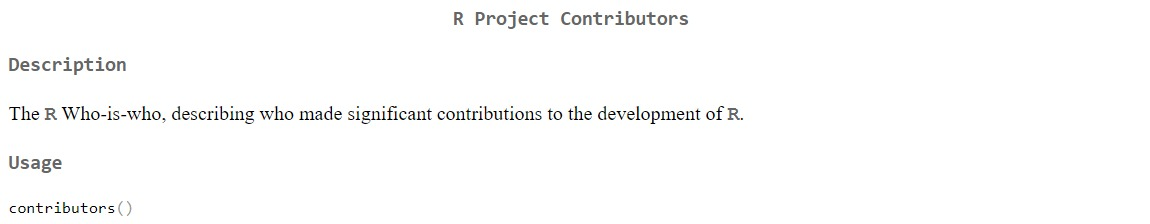
\includegraphics[width=0.8\linewidth]{images/Help.jpeg}
\caption{\label{fig:help_image}Help de la función contributors()}
\end{figure}

\item 
Con la función getwd, se mostrará en pantalla el directorio actual de trabajo, en 
el cual se buscan los archivos que llamamos en el resto de funciones que cargan archivos.

\begin{Schunk}
\begin{Sinput}
> getwd()
\end{Sinput}
\end{Schunk}


\item 
Con la función setwd, podemos cambiar el directorio actual de trabajo. Necesita
recibir como parámetro una cadena de texto con la dirección absoluta del nuevo directorio
de trabajo.

\begin{Schunk}
\begin{Sinput}
> setwd("C:NuevoDirectorio")
\end{Sinput}
\end{Schunk}


\item 
En el caso de querer visualizar en consola los archivos que se pueden encontrar en el
directorio de trabajo, es necesario llamar a la función list.files. También podemos llamar a
la función dir(), la cual muestra también los archivos.

\begin{Schunk}
\begin{Sinput}
> list.files()
> dir()
\end{Sinput}
\end{Schunk}


\item
Si queremos ver todos los paquetes que podemos cargar en R, podemos llamar a la función library
sin ningún parámetro.

\begin{Schunk}
\begin{Sinput}
> library()
\end{Sinput}
\end{Schunk}


Aparte, si queremos ver todos los paquetes ya cargados, podemos llamar a estas funciones:

\begin{Schunk}
\begin{Sinput}
> getOption("defaultPackages")
\end{Sinput}
\begin{Soutput}
[1] "datasets"  "utils"     "grDevices" "graphics"  "stats"     "methods"  
[7] "arules"   
\end{Soutput}
\end{Schunk}


La primera función muestra los nombres de los paquetes que se quieren cargar al iniciar la terminal de R, y la segunda muestra los paquetes efectivamente cargados.
Se puede visualizar todas las funciones que contiene un paquete si añadimos la opción help con
su nombre. Por ejemplo, para el paquete base:

\begin{Schunk}
\begin{Sinput}
> library(help="base")
> search()
\end{Sinput}
\end{Schunk}

Aparte, podemos cargar paquetes con library si pasamos como argumento el nombre de dicho paquete.

\begin{Schunk}
\begin{Sinput}
> library(class)
\end{Sinput}
\end{Schunk}


\end{enumerate}

\subsection{Explicación de la instalación e importación de paquetes en R}

\begin{enumerate}

\item 
La manera más básica de instalar paquetes es, desde la gui de R, ir a la opción Paquetes -> Seleccionar espejo CRAN... y escoger el espejo que nos interesa, en nuestro caso, el espejo Spain (Madrid)
\begin{figure}[H]
\centering
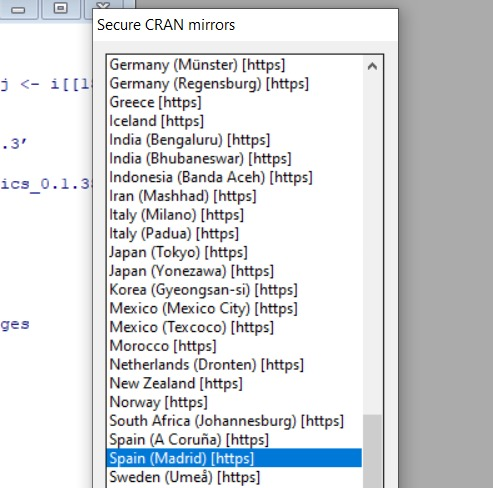
\includegraphics[width=0.5\linewidth]{images/cran_mirror.jpeg}
\caption{\label{fig:cran_mirror_image}Repositorio CRAN España (Madrid)}
\end{figure}
Después nos vamos a la opción Paquetes -> cargar paquete, y podemos encontrar una lista de los paquetes que podemos instalar a partir de este espejo CRAN
\begin{figure}[H]
\centering
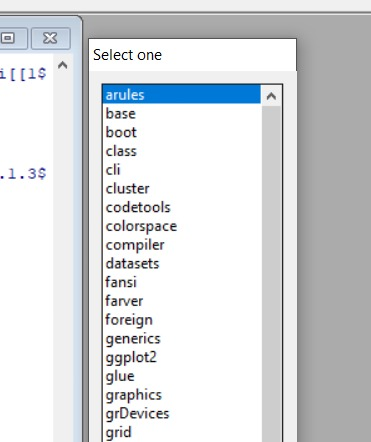
\includegraphics[width=0.5\linewidth]{images/cran_mirror_packages.jpeg}
\caption{\label{fig:cran_mirror_packages}Paquetes disponibles en el repositorio CRAN España (Madrid)}
\end{figure}

\item 
Si queremos instalar un paquete a partir de un repositorio, podemos llamar a install.packages
O bien lo instalamos de un repositorio (una vez se llame, pedirá escojer un repositorio, por defecto
elegiremos CRAN de Spain, Madrid):

\begin{Schunk}
\begin{Sinput}
> install.packages("nombre del paquete a instalar")
\end{Sinput}
\end{Schunk}

También podemos descargar el archivo zip de un paquete, y abrirlo con install.packages, indicando que no lo descargamos de ningún repositorio con repos=NULL. Podemos encontrar el paquete ggplot2 en este enlace: \href{https://cran.r-project.org/web/packages/ggplot2/index.html}{ggplot2}
Todos los paquetes que descarguemos los guardaremos en una carpeta C:/tmp, dentro de la raíz del disco:

\begin{Schunk}
\begin{Sinput}
> install.packages("C:/tmp/ggplot2_3.4.3.zip", repos=NULL)
> library(ggplot2)
\end{Sinput}
\end{Schunk}

Seguramente este paquete instalado dependerá de otros paquetes para poder ser utilizado. En ese caso, instalaremos
los paquetes necesarios que se nos indique al intentar cargarlo con library, con la técnica anterior, utilizando install.packages del repositorio CRAN que escogimos anteriormente:

\begin{Schunk}
\begin{Sinput}
> install.packages("gtable")
> install.packages("scales")
> install.packages("vctrs")
> install.packages("tibble")
> install.packages("withr")
> library(ggplot2)
\end{Sinput}
\end{Schunk}

Para esta práctica, nosotros vamos a instalar también este paquete: \href{https://cran.r-project.org/web/packages/arules/index.html}{arules}

\begin{Schunk}
\begin{Sinput}
> install.packages("C:/tmp/arules_1.7-6.zip", repos=NULL)
> library(arules)
\end{Sinput}
\end{Schunk}

Nos notificará al cargarlo con library de que necesita el paquete generics. Lo instalaremos y después cargaremos otra vez arules. Debería funionar

\begin{Schunk}
\begin{Sinput}
> install.packages("generics")
> library(arules)
\end{Sinput}
\end{Schunk}


\item
Por ahora hemos instalado todos los paquetes que necesitaremos para hacer los ejercicios. El problema es que, cuando cerremos la terminal de R y la volvamos a abrir, será necesario volver a llamar a library(arules) y library(ggplot2) si queremos utilizar ambos paquetes. Para cargar estos paquetes nada más abir la terminal, vamos a movernos al siguiente directorio, con el explorador de archivos
\begin{verbatim}
C:\Program Files\R\R-4.3.1\library\base\R
\end{verbatim}
Lo siguiente que haremos es copiar el archivo llamado Rprofile, y lo pegaremos en un directorio accesible, como puede ser el escritorio. Ahora lo abrimos con un editor de texto, y nos dirigimos a la línea 46, o buscamos la palabra R\_DEFAULT\_PACKAGES. Podemos encontrar lo siguiente:
\begin{figure}[H]
\centering
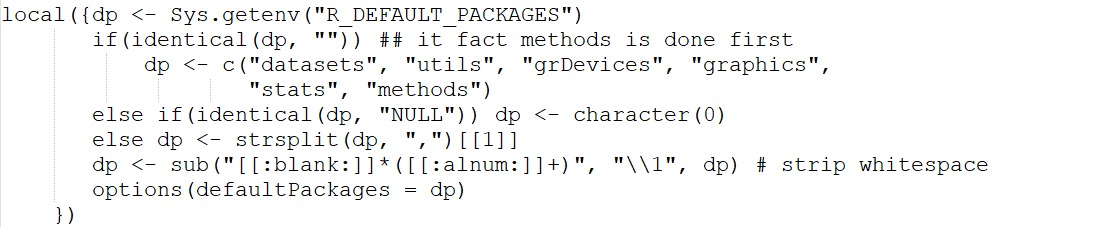
\includegraphics[width=0.8\linewidth]{images/Default_packages.jpeg}
\caption{\label{fig:default_packages}Archivo Rprofile}
\end{figure}
Lo que haremos es, al array dp, que se le asigna como valor una c() con los nombres de los paquetes que se cargan al iniciar la terminal, añadiremos los paquetes que deseemos importar. En nuestro caso, añadiremos por ahora solamente arules. La variable dp quedará de la siguiente forma:
\begin{verbatim}
dp <- c("datasets", "utils", "grDevices", "graphics", "stats",
"methods", "arules")
\end{verbatim}
Para terminar, guardaremos este archivo, y lo volveremos a mover al directorio base de R, sobreescribiendo el archivo original
Para comprobar que se ha cargado correctamente, llamaremos a la función getOption("defaultPackages"), y efectivamente debería aparecer arules. También podemos comprobarlo con search()

\end{enumerate}

\subsection{Explicación de la generación de artículos científicos con LaTex y Sweave}

\begin{enumerate}

\item
LaTex es un sistema de preparación de documentos para composición de texto, permitiendo generar documentos de extensión pdf con un formato de artículo científico, entre otros. Algunas de las anotaciones básicas en LaTex son:
\begin{verbatim}
\documentclass[a4paper]{article} -> El formato del documento 
será un artículo

\title{Titulo} -> Establece el título del documento como 
"Titulo"

\author{Friedrich} -> Establece como autor del documento a 
"Friedrich"

\begin{document} -> Indica el inicio del documento 

\maketitle -> Genera dentro del cuerpo del documento el
título

\texttt{Texto} -> Genera un cuadro de texto, con el contenido
"Texto", justificado

\end{document} -> Indica el fin del documento 
\end{verbatim}

\item
Sweave es un componente del lenguaje de programación R que permite la integración de código en documentos escritos con LaTex. Podemos encontrar algunos ejemplos de archivos en este directorio:
\begin{verbatim}
C:\Program Files\R\R-4.3.1\library\utils\Sweave
\end{verbatim}
Vamos a abrir, por ejemplo, el archivo example-1.Rnw:
\begin{figure}[H]
\centering
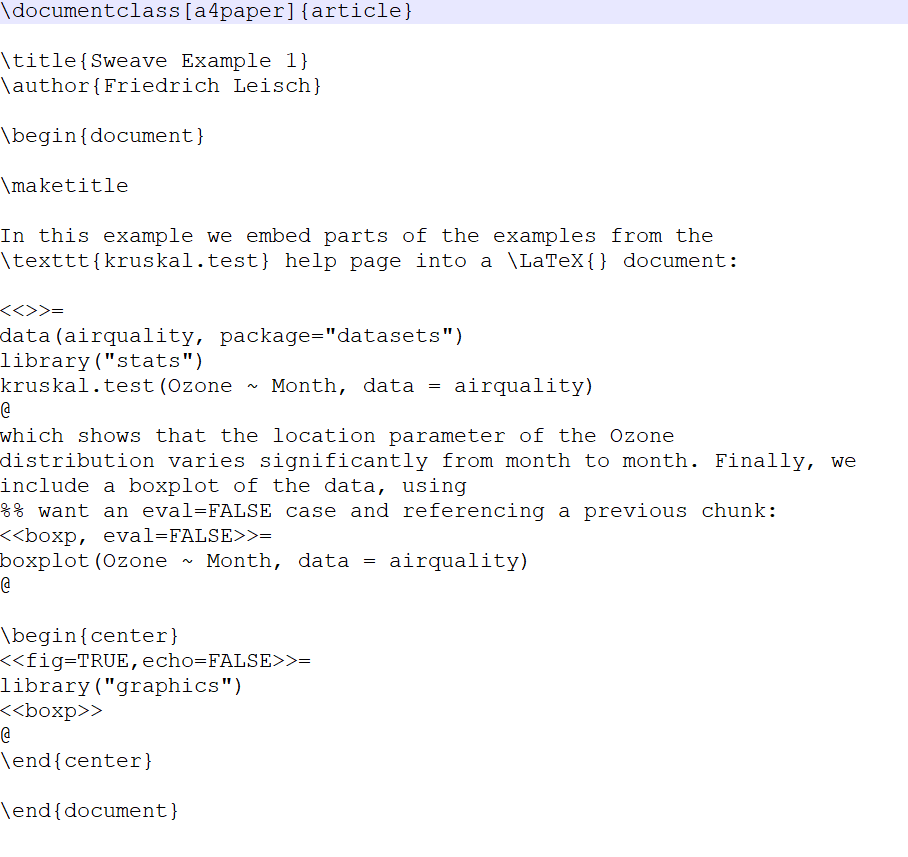
\includegraphics[width=0.5\linewidth]{images/example-1.Rnw.PNG}
\caption{\label{fig:example_rnw}example-1.Rnw}
\end{figure}
Podemos observar que, a parte de las anotaciones de LaTex que podemos encontrar, también están unas anotaciones con los siguientes símbolos <<>>= y @:
\newline
\begin{verbatim}
<<>> =
data(airquality, package="datasets")
library("stats")
kruskal.test(Ozone ~ Month, data = airquality)
\@
\end{verbatim}
Estas son anotaciones especiales de Sweave, que nos permitirán anclar a nuestro documento líneas de código y su resultado al ejecutarlas con R.
Para generar un documento pdf con LaTex con Sweave, a partir del archivo, podemos llamar a las siguientes funciones:

\begin{Schunk}
\begin{Sinput}
> rnwfile <- system.file("Sweave", "example-1.Rnw", package="utils") 
> Sweave(rnwfile) 
> tools::texi2pdf("example-1.tex")
\end{Sinput}
\end{Schunk}

Al ejecutarlo, nos saldrá un error, ya que necesitamos el compilador de LaTex.

\item
Vamos a instalar MiKTeX. Para ello, primero descargaremos el instalador, que podemos encontrar en este enlace: \href{https://miktex.org/download}{MiKTex}
Durante la instalación, aceptamos los términos de copyright, y elegimos instalar MiKTeX sólo para el usuario actual. Vamos a instalar MiKTeX en el directorio que nos aparece. El tamaño del papel será A4. Para la opción de instalar los paquetes que falten al vuelo, elegimos la opción Yes, ya que, sino, nos preguntará todo el rato cada paquete que queramos instalar. Finalmente, comenzamos la instalación, y esperamos a que finalice.

\item
Si volvemos a abrir una nueva terminal y a llamar a las funciones de antes, se acabará generando el documento en extensión pdf.
Podremos encontrar el archivo pdf dentro de nuestro directorio de trabajo.
Al abrirlo, podremos ver que, efectivamente, su contenido ha sido generado por el archivo .Rnw que hemos utilizado de ejemplo
\begin{figure}[H]
\centering
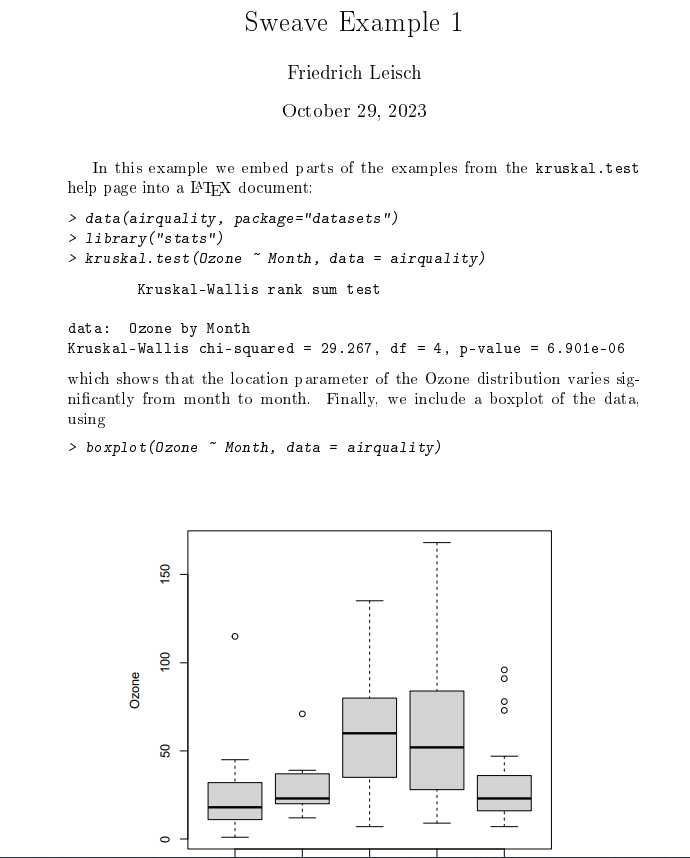
\includegraphics[width=0.5\linewidth]{images/sweave_generado.PNG}
\caption{\label{fig:archivo_generado_latex_sweave}Archivo pdf generado con LaTex y Sweave}
\end{figure}

\end{enumerate}

\section{Parte 1}

En este ejercicio, vamos a comentar la resolución, vista en clase de laboratorio, de cada uno de los cuatro apartados de la práctica.

\subsection{Ejercicio 1.1}

Lo primero que tenemos que hacer es crear el archivo con el conjunto de datos, dentro del directorio de trabajo. Crearemos un archivo .txt llamado Urano.txt
Tenemos que asegurarnos de escribirlo siguiendo estas reglas:

\begin{enumerate}

\item
Debe haber una columna que numere las filas, excepto en la primera fila, que solamente dejaremos una tabulación 

\item
En la primera fila dejamos una tabulación y escribimos el nombre de las variables 

\item
La utilización de los ; no es lo mismo que en números decimales, utilizamos un punto ('.')

\item
Por último, no dejar ningún nombre de variable con espacios en blanco 

\end{enumerate}

El archivo quedará entonces de la siguiente manera:

\begin{figure}[H]
\centering
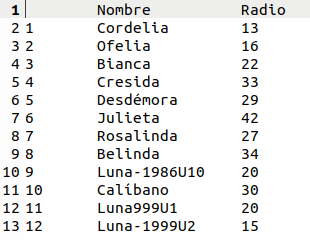
\includegraphics[width=0.5\linewidth]{images/Image1.png}
\caption{\label{fig:archivo_urano_txt}Archivo Urano.txt}
\end{figure}

Lo siguiente que hay que hacer es cargar el archivo. Para ello, escribimos la siguiente función:
%no pongo nombre de nodo y EVAL=false para que se vea la tabla

\begin{Schunk}
\begin{Sinput}
> s<-read.table("Urano.txt")
> s
\end{Sinput}
\begin{Soutput}
         Nombre Radio
1      Cordelia    13
2        Ofelia    16
3        Bianca    22
4       Cresida    33
5     Desdémora    29
6       Julieta    42
7     Rosalinda    27
8       Belinda    34
9  Luna-1986U10    20
10     Calíbano    30
11    Luna999U1    20
12  Luna-1999U2    15
\end{Soutput}
\end{Schunk}


Podremos ver que se ha cargado la tabla. Para ver las dimensiones de la tabla, hacemos:

\begin{Schunk}
\begin{Sinput}
> dim(s)
\end{Sinput}
\begin{Soutput}
[1] 12  2
\end{Soutput}
\end{Schunk}


Ahora queremos ordenar de menor a mayor los valores de la columna Radio. Para ello, tenemos que hacer lo siguiente:

\begin{Schunk}
\begin{Sinput}
> so=s[order(s$Radio),]
> so
\end{Sinput}
\begin{Soutput}
         Nombre Radio
1      Cordelia    13
12  Luna-1999U2    15
2        Ofelia    16
9  Luna-1986U10    20
11    Luna999U1    20
3        Bianca    22
7     Rosalinda    27
5     Desdémora    29
10     Calíbano    30
4       Cresida    33
8       Belinda    34
6       Julieta    42
\end{Soutput}
\end{Schunk}


Es necesario para ello poner que tomamos el atributo Radio con un dólar. Escribimos dicho  valor en el primer elemento de la lista, ya que queremos ordenar por filas.
Si queremos obtener la misma tabla pero con orden invertido, necesitamos llamar a la función rev() de esta manera:

\begin{Schunk}
\begin{Sinput}
> so=s[rev(order(s$Radio)),]
> so
\end{Sinput}
\begin{Soutput}
         Nombre Radio
6       Julieta    42
8       Belinda    34
4       Cresida    33
10     Calíbano    30
5     Desdémora    29
7     Rosalinda    27
3        Bianca    22
11    Luna999U1    20
9  Luna-1986U10    20
2        Ofelia    16
12  Luna-1999U2    15
1      Cordelia    13
\end{Soutput}
\end{Schunk}


Con estos datos que hemos cargado, vamos a empezar a analizar los datos, obteniendo el rango, las frecuencias absolutas y relativas (también las acumuladas), la moda, la media aritmética, la desviación típica, la varianza (poblacional) y los cuartiles, de la columna Radio de nuestra tabla de Urano:

Para calcular el rango, podemos hacer la siguiente operación:

\begin{Schunk}
\begin{Sinput}
> max(s$Radio) - min(s$Radio)
\end{Sinput}
\begin{Soutput}
[1] 29
\end{Soutput}
\end{Schunk}


Existe una función range la cual nos muestra por pantalla este valor máximo y mínimo en vez de calcularnos el valor del rango

\begin{Schunk}
\begin{Sinput}
> range(s$Radio)
\end{Sinput}
\begin{Soutput}
[1] 13 42
\end{Soutput}
\end{Schunk}


Ahora, para no tener que estar llamando todo el rato a la columna Radio de la tabla r, vamos a crear la siguiente variable:

\begin{Schunk}
\begin{Sinput}
> R<-s$Radio
\end{Sinput}
\end{Schunk}


Ya que la función rango no está implementada, la vamos a implementar nosotros. Para crear una función, tenemos que definirla con la siguiente sintaxis: $nombre\_funcion <- function(parametros\_separados\_comas) \{ cuerpo\_codigo \}$

Nuestra implementación para calcular el rango será la siguiente:

\begin{Schunk}
\begin{Sinput}
> rango = function( Radio ){ max(Radio)-min(Radio) }
\end{Sinput}
\end{Schunk}


Una vez pulsemos Enter, podremos utilizar esta función. El problema es que, una vez cerremos la conslola y la volvamos a abrir, la función se habrá perdido y ya no podrá ser llamada. Para guardarla, tenemos que llamar a la función dump de la siguiente manera:

\begin{Schunk}
\begin{Sinput}
> dump("rango",file="rango.R") 
\end{Sinput}
\end{Schunk}


Si llamamos a la función list.files(), podemos observar que se ha creado en el directorio de trabajo el archivo rango.R, que es donde se ha guardado al implementación de nuestra función. Si llegamos a cerrar la terminal y la volvemos a arbrir, tendremos que cargar esta función con la función source():

\begin{Schunk}
\begin{Sinput}
> source("rango.R") 
> rango(R)
\end{Sinput}
\begin{Soutput}
[1] 29
\end{Soutput}
\end{Schunk}


Podemos comprobar que, si tomamos el menor valor, que es 13, y el mayor valor, que es 42, al hacer la resta, obtenemos 29, como hemos visto en clase

Para obtener una tabla con las frecuencias absolutas de los elementos de una tabla, tenemos que cambiar el formato de la tabla, con la función table

\begin{Schunk}
\begin{Sinput}
> frecabsradio<-table(R)
> frecabsradio
\end{Sinput}
\begin{Soutput}
R
13 15 16 20 22 27 29 30 33 34 42 
 1  1  1  2  1  1  1  1  1  1  1 
\end{Soutput}
\end{Schunk}


Los valores de las frecuencias coinciden con las vistas en clase

Para obtener la frecuencia absoluta acumulada, necesitamos llamar a la función cumsum() de la tabla:

\begin{Schunk}
\begin{Sinput}
> frecabsacumradio<-cumsum(frecabsradio)
> frecabsacumradio
\end{Sinput}
\begin{Soutput}
13 15 16 20 22 27 29 30 33 34 42 
 1  2  3  5  6  7  8  9 10 11 12 
\end{Soutput}
\end{Schunk}


No existe una función en R para calcular la tabla con las frecuencias relativas. Vamos a crear una implementación propia:

\begin{Schunk}
\begin{Sinput}
> frecrel=function(Radio){ table(Radio)/length(Radio) }
> frecrel(R)
\end{Sinput}
\begin{Soutput}
Radio
        13         15         16         20         22         27         29 
0.08333333 0.08333333 0.08333333 0.16666667 0.08333333 0.08333333 0.08333333 
        30         33         34         42 
0.08333333 0.08333333 0.08333333 0.08333333 
\end{Soutput}
\end{Schunk}


Los valores de las frecuencias coinciden con las vistas en clase

Podemos aprovechar a crear una función que calcule las frecuencias relativas acumuladas utilizando cumsum:

\begin{Schunk}
\begin{Sinput}
> frecrelacum=function(Radio){ cumsum(table(Radio))/length(Radio) }
> frecrelacum(R)
\end{Sinput}
\begin{Soutput}
        13         15         16         20         22         27         29 
0.08333333 0.16666667 0.25000000 0.41666667 0.50000000 0.58333333 0.66666667 
        30         33         34         42 
0.75000000 0.83333333 0.91666667 1.00000000 
\end{Soutput}
\end{Schunk}


Los valores de las frecuencias coinciden con las vistas en clase

Si queremos calcular la moda, no existe en R ningún paquete por defecto que implemente la moda directamente. Para obtenerla, vamos instalar el paquete DescTools, y lo cargaremos con library: 

\begin{Schunk}
\begin{Sinput}
> install.packages("DescTools")
> library(DescTools)
\end{Sinput}
\end{Schunk}



\begin{Schunk}
\begin{Soutput}
package ‘DescTools’ successfully unpacked and MD5 sums checked

The downloaded binary packages are in
	C:\Users\Alvaro\AppData\Local\Temp\RtmpWokKcS\downloaded_packages
\end{Soutput}
\end{Schunk}


Para calcular la moda, llamaremos a la función Mode(), pasando como argumento la columna Radio:

\begin{Schunk}
\begin{Sinput}
> moda<-Mode(R)
> moda
\end{Sinput}
\begin{Soutput}
[1] 20
attr(,"freq")
[1] 2
\end{Soutput}
\end{Schunk}


Al igual que en teoría, el valor que más veces se repite es el 20

Para saber el número de elementos que tiene una lista, podemos utilizar la función length():

\begin{Schunk}
\begin{Sinput}
> length(R)
\end{Sinput}
\begin{Soutput}
[1] 12
\end{Soutput}
\end{Schunk}


Ahora vamos a calcular la media aritmética de los valores. En R hay una función implementada que ya nos calcula la media, mean(), a la cual pasaremos como argumento la columna Radio:

\begin{Schunk}
\begin{Sinput}
> mean(R)
\end{Sinput}
\begin{Soutput}
[1] 25.08333
\end{Soutput}
\end{Schunk}


Si utilizamos la función de la media aritmética vista en clase, obtenemos el mismo resultado

\begin{figure}[H]
\centering
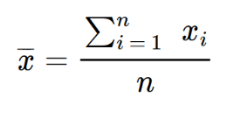
\includegraphics[width=0.3\linewidth]{images/formula_media_aritmetica.png}
\caption{\label{fig:formula_media_aritmetica}Fórmula de la media aritmética, vista en clase}
\end{figure}

$\overline{x} = \frac{13+16+22+33+29+42+27+34+20+30+20+15}{12} = \frac{301}{12} = 25,0833$

Ahora vamos a calcular la desviación típica. Para ello, utilizaremos la función sd(), pasando como argumento la columna Radio:

\begin{Schunk}
\begin{Sinput}
> sd(R)
\end{Sinput}
\begin{Soutput}
[1] 8.857029
\end{Soutput}
\end{Schunk}


Aplicando la fórmula vista en clase:

\begin{figure}[H]
\centering
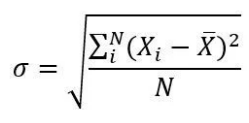
\includegraphics[width=0.3\linewidth]{images/formula_desviacion_tipica.png}
\caption{\label{fig:formula_desviacion_tipica}Fórmula de la desviación típica, vista en clase}
\end{figure}

$\sigma = \sqrt{\frac{(13-25,0833)^{2}+(16-25,0833)^{2}+...+(20-25,0833)^{2}+(15-25,0833)^{2}}{12}} = \sqrt{\frac{10}{12}} = 8,47996$

Si hacemos las cuentas tal y como hemos visto en clase, podremos observar que los resultados no coinciden (el resultado nos da  8,857029 con la función sd(), y 8,47996 haciendo los cálculos con la fórmula). ¿Qué está pasando?

La función sd() devuelve la desviación típica en función de n-1, mientras que la fórmula vista en teoría la devuelve en función de n. Podemos ver esta información en la sección de detalles al llamar a help(sd)

\begin{figure}[H]
\centering
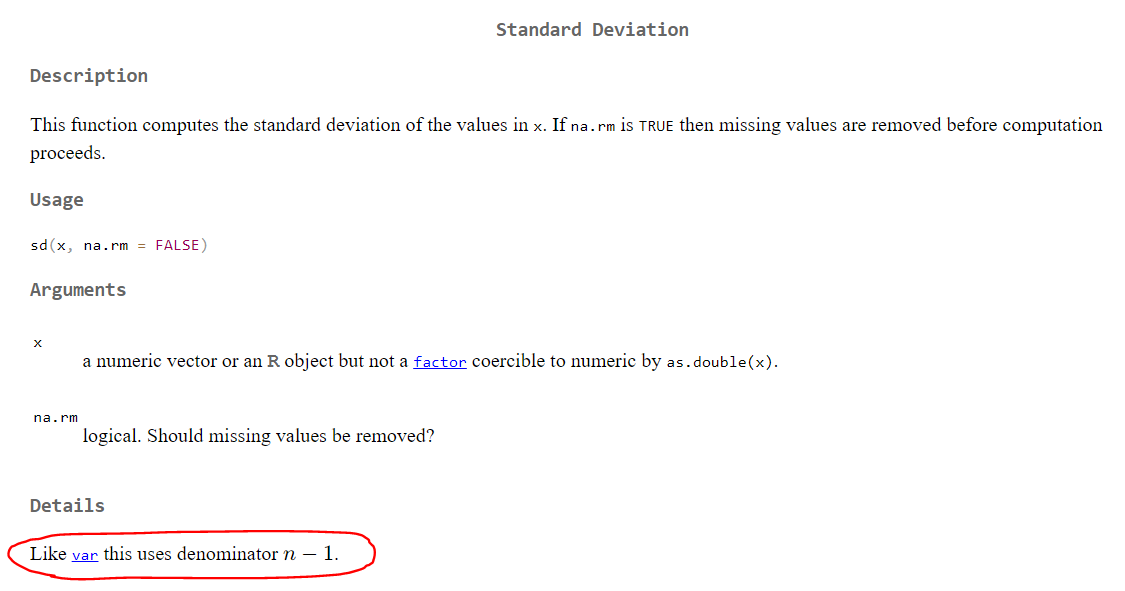
\includegraphics[width=0.8\linewidth]{images/sd_help.PNG}
\caption{\label{fig:help_de_sd}Help de sd()}
\end{figure}

En resumen, el denominador que utiliza es n-1, siendo n el número de elementos que se encuentren en la lista pasada como argumento. Para calcular nuestra desviación típica poblacional, necesitaremos implementar la siguiente función, la cual cambia el denominador con el que se obtiene la desviación:


\begin{Schunk}
\begin{Sinput}
> sdp <- function(x){ sqrt( (sd(x)^2) * ((length(x)-1)/length(x)) ) }
> sdp(R)
\end{Sinput}
\begin{Soutput}
[1] 8.47996
\end{Soutput}
\end{Schunk}


Ahora, como podemos observar, los cálculos si que son los de la desviación típica poblacional

Si queremos calcular la varianza, tenemos que utilizar la función var(), pasando como argumento la columna Radio:


\begin{Schunk}
\begin{Sinput}
> var(R)
\end{Sinput}
\begin{Soutput}
[1] 78.44697
\end{Soutput}
\end{Schunk}


Nos va a ocurrir lo mismo que nos ha pasado con la desviación típica, por lo que vamos a implementar la siguiente función:


\begin{Schunk}
\begin{Sinput}
> varp <- function(x){ var(x) * ((length(x)-1)/length(x)) }
> varp(R)
\end{Sinput}
\begin{Soutput}
[1] 71.90972
\end{Soutput}
\end{Schunk}


Ahora vamos a calcular la mediana. La metodología vista en clase es, primero ordenar los datos de manera ascendente, y después aplicar el siguiente criterio para obtener la mediana:

\begin{figure}[H]
\centering
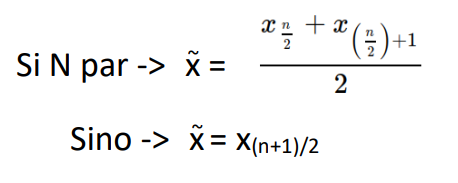
\includegraphics[width=0.3\linewidth]{images/formula_mediana.png}
\caption{\label{fig:formula_mediana}Fórmula de la mediana, vista en clase}
\end{figure}

Con esta expresión, sabemos que N es par, por tanto la mediana será la media aritmética de los dos valores en el centro de la lista de valores ordenados: 13, 15, 16, 20, 20, 22, 27, 29, 30, 33, 34, 42. El resultado será $\frac{22+27}{2} = 24,5$

Podemos calcular la mediana con la función median(), pasando como argumento la columna Radio

\begin{Schunk}
\begin{Sinput}
> median(R)
\end{Sinput}
\begin{Soutput}
[1] 24.5
\end{Soutput}
\end{Schunk}


Para terminar, calculamos los cuartiles. Según lo visto en clase, el criterio para calcular los cuartiles es el siguiente:

\begin{figure}[H]
\centering
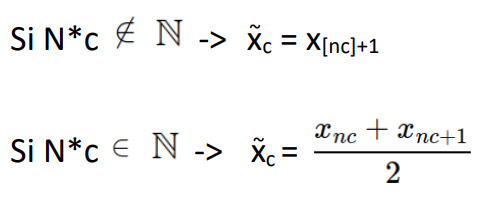
\includegraphics[width=0.3\linewidth]{images/formula_cuartiles.png}
\caption{\label{fig:formula_cuartiles}Fórmula de los cuartiles, vista en clase}
\end{figure}

Para el primer cuartil, 12*0,25 = 3, como es un número entero, este cuantil es igual a la media aritmética de los elementos en las posiciones 3 y 4, siendo el resultado $\frac{16+20}{2} = 19$

Para el tercer cuartil, ocurre lo mismo, pero la media aritmética es para los elementos en las posiciones 9 y 10, siendo el resultado $\frac{30+33}{2} = 31,5$

Para calcular los cuartiles en R, utilizaremos la función quantile(). Es necesario pasar como primer argumento la columna Radio, y como segundo argumento la posición del cuartil (por ejemplo, en 0.25, el cuartil se encuentra en el 25\%):

\begin{Schunk}
\begin{Sinput}
> (cuartil1<-quantile(s$Radio,0.25))
\end{Sinput}
\begin{Soutput}
25% 
 19 
\end{Soutput}
\begin{Sinput}
> (cuartil2<-quantile(s$Radio,0.5))
\end{Sinput}
\begin{Soutput}
 50% 
24.5 
\end{Soutput}
\begin{Sinput}
> (cuartil3<-quantile(s$Radio,0.75))
\end{Sinput}
\begin{Soutput}
  75% 
30.75 
\end{Soutput}
\end{Schunk}


Los resultados no coinciden exactamente con los vistos en teoría, pero son prácticamente los mismos

Podríamos haber puesto los valores 0.1, 0.2, ..., 0.9 para obtener los deciles, y valores desde el 0.01, que van incrementando en 0.01, hasta 0.99, para obtener los percentiles. Lo equivalente a lo visto en clase sería lo siguiente:

\begin{figure}[H]
\centering
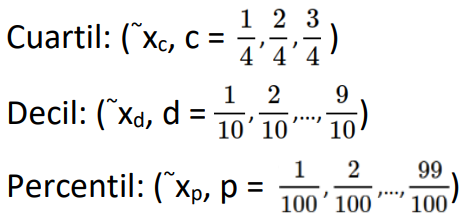
\includegraphics[width=0.3\linewidth]{images/expresion_cuartiles_deciles_percentiles.png}
\caption{\label{fig:expresion_cuartiles}Expresión de cuartiles, deciles y percentiles vista en clase}
\end{figure}

Con esto, ya hemos terminado el análisis descriptivo de los datos

\subsection{Ejercicio 1.2}

En este apartado realizamos un ejercicio visto en clase de análisis de asociación de datos en R con el algoritmo A Priori. 

Primero, cargamos librería arules que contiene algoritmo apriori.


\begin{Schunk}
\begin{Sinput}
> library("arules")
\end{Sinput}
\end{Schunk}


Procedemos ahora a cargar la matriz de asociaciones, etiquetada con sus
cabeceras.


\begin{Schunk}
\begin{Sinput}
> muestra<-Matrix(c(1,1,0,1,1, 1,1,1,1,0, 1,1,0,1,0, 1,0,1,1,0, 1,1,0,0,0, 0,0,0,1,0),
+ 6, 5, byrow=TRUE, dimnames=list(
+ c("suceso1", "suceso2", "suceso3", "suceso4", "suceso5", "suceso6"),
+ c("Pan", "Agua", "Cafe", "Leche", "Naranjas")),
+ sparse=TRUE )
\end{Sinput}
\end{Schunk}


Antes de poder emplear el algoritmo apriori, tenemos que convertir la matriz
a un objeto de transacciones a traves de una matriz dispersa.


\begin{Schunk}
\begin{Sinput}
> muestrangCMatrix<-as(muestra,"nsparseMatrix")
\end{Sinput}
\end{Schunk}



\begin{Schunk}
\begin{Sinput}
> traspmuestrangCMatrix<-t(muestrangCMatrix)
\end{Sinput}
\end{Schunk}



\begin{Schunk}
\begin{Sinput}
> transacciones<-as(traspmuestrangCMatrix,"transactions")
\end{Sinput}
\end{Schunk}


En teoría, para implementar el algoritmo, tendríamos que seguir los siguientes pasos:

Paso A: Se calcula el soporte, considerando que la medida es antimonótona. Si el suceso es frecuente y su soporte supera el umbral (en nuestro caso, utilizaremos s = 50\%), todos los subconjuntos de dicho conjunto son también frecuentes, ya que su soporte es mayor o igual que el del conjunto que los contiene

Este paso se divide en dos subpasos:

Paso A.1: Se pasa por sucesos elementales para calcular su soporte y se eliminan los que no alcancen el umbral fijado

El soporte se expresa como: 

$\forall\{A_{i}\}_{i=1}^{\infty}\subset P(E) $ con $ A_{i} \cap A_{j} = \emptyset$ $\forall$ i != j, s:$P(E)$ ->  $ R+ / S(A_{i} \cup A_{j}) = \frac{n_{A_{i} \cup A_{j}}}{n_{T}}$

s(\{Pan\}) = $\frac{n_{A_{i} \cup A_{j}}}{n_{T}}$ = $\frac{5}{6}$ = 83,33\% > 50\% -> supera el umbral s
\newline
s(\{Agua\}) = $\frac{4}{6}$ = 66,67\% > 50\% -> supera el umbral s
\newline
s(\{Café\}) = $\frac{2}{6}$ = 33,33\% < 50\% -> no supera el umbral s
\newline
s(\{Leche\}) = $\frac{5}{6}$ = 83,33\% > 50\% -> supera el umbral s
\newline
s(\{Naranjas\}) = $\frac{1}{6}$ = 16,67\% < 50\% -> no supera el umbral s

Los sucesos elementales \{Café\} y \{Naranjas\} quedan descartados como posibles sucesos elementales pertenecientes a sucesos mayores que lleguen o superen el umbral de soporte.

Paso A.2: Dos pasos sucesivos en cada dimensión, comentando subconjuntos de 2 elementos y
terminando cuando ninguno llega al soporte umbral

Paso A.2.1: Se utiliza A priori-gen para identificar sucesos candidatos. Se utiliza una base de subconjunto para la dimensión anterior con el método $F_{k-1}* F_{k-1}$ se obtiene el conjunto de candidatos en la dimensión k, uniendo pares de conjuntos candidatos de la dimensión anterior k-1, pero sólo aquellos pares en los que coinciden sus dos primeros k-2 elementos
Sean A = \{$a_1, a_2, ..., a_{k-1}$\} y B = \{$b_1, b_2, ..., b_{k-1}\}$, dos sucesos frecuentes identificados en dimensión k-1 A y B sólo se unirán en k si cumplen:

\begin{enumerate}
    \item $a_j$ = $b_j$ para todo j = 1, 2, ..., k - 2
    \item $a_{k-1}$ = $b_{k-1}$
\end{enumerate}

Para k = 2:

\{Pan\}\quad\quad\quad\quad\{Pan, Agua\}
\newline
\{Agua\}\quad->\quad\{Pan, Leche\}
\newline
\{Leche\}\quad\quad\quad\{Agua, Leche\}

Para k = 3:

\{Pan, Agua\}
\newline
\{Pan, Leche\}\quad->\quad\{Pan, Agua, Leche\}
\newline
\{Agua, Leche\}

Paso A.2.2: Calcular el soporte de los sucesos identificados en el paso A.2.1. Dividido en 3 subpasos:

Paso A.2.2.1: Partición de los sucesos candidatos en el hash tree

Antes de empezar con este paso, es necesario numerar todos los sucesos. Empezamos numerando todos los sucesos elementales, incluidos aquellos que no superaron el umbral de soporte:

\{Pan\} = 1, \{Agua\} = 2, \{Café\} = 3,  \{Leche\} = 4,  \{Naranjas\} = 5, 

Una vez numerados los sucesos elementales, numeramos los otros sucesos candidatos que hemos formado con el algoritmo K${-1}$*K${-1}$:

\{Pan, Agua\} = 6, \{Pan, Leche\} = 7, \{Agua, Leche\} = 8, \{Pan, Agua, Leche\} = 9

Una vez numerados, podemos empezar a hacer las particiones. Empezamos con los sucesos candidatos, agrupándolos para el tamaño 2:

\begin{figure}[H]
\centering
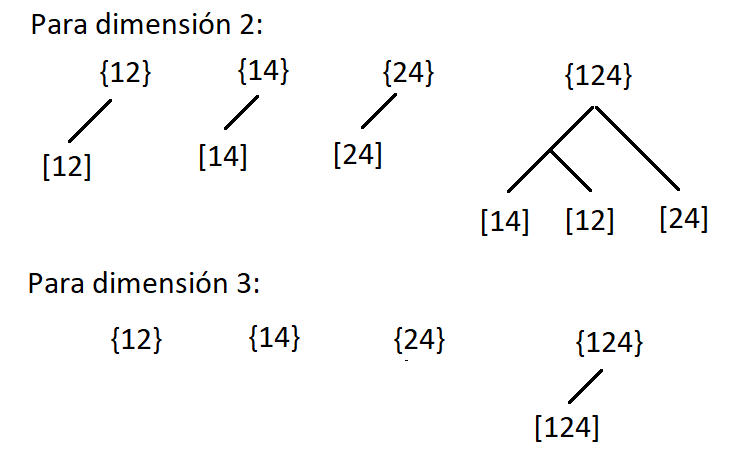
\includegraphics[width=0.8\linewidth]{images/apriori_candidatos_1.png}
\caption{\label{fig:apriori_sucesos_candidatos}Hash tree sucesos candidatos}
\end{figure}

Paso A.2.2.2: Partición de los sucesos de la muestra en el hash tree

\begin{figure}[H]
\centering
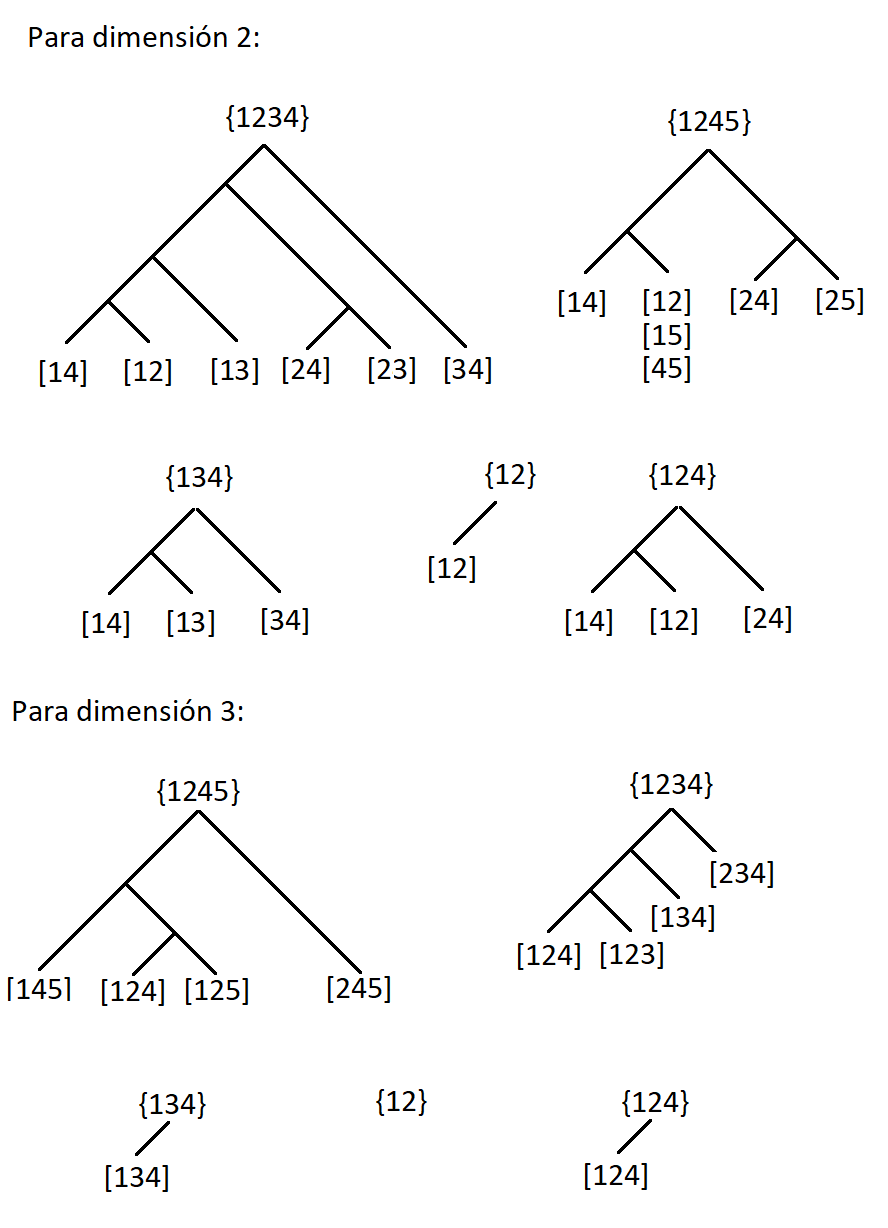
\includegraphics[width=0.8\linewidth]{images/apriori_muestras_1.png}
\caption{\label{fig:apriori_sucesos_muestra}Hash tree sucesos muestra}
\end{figure}

Paso A.2.2.3: Comparación de ambas particiones. Todas las hojas coincidentes incrementan 1 unidad el numerador en el cálculo del soporte calculado:

\begin{figure}[H]
\centering
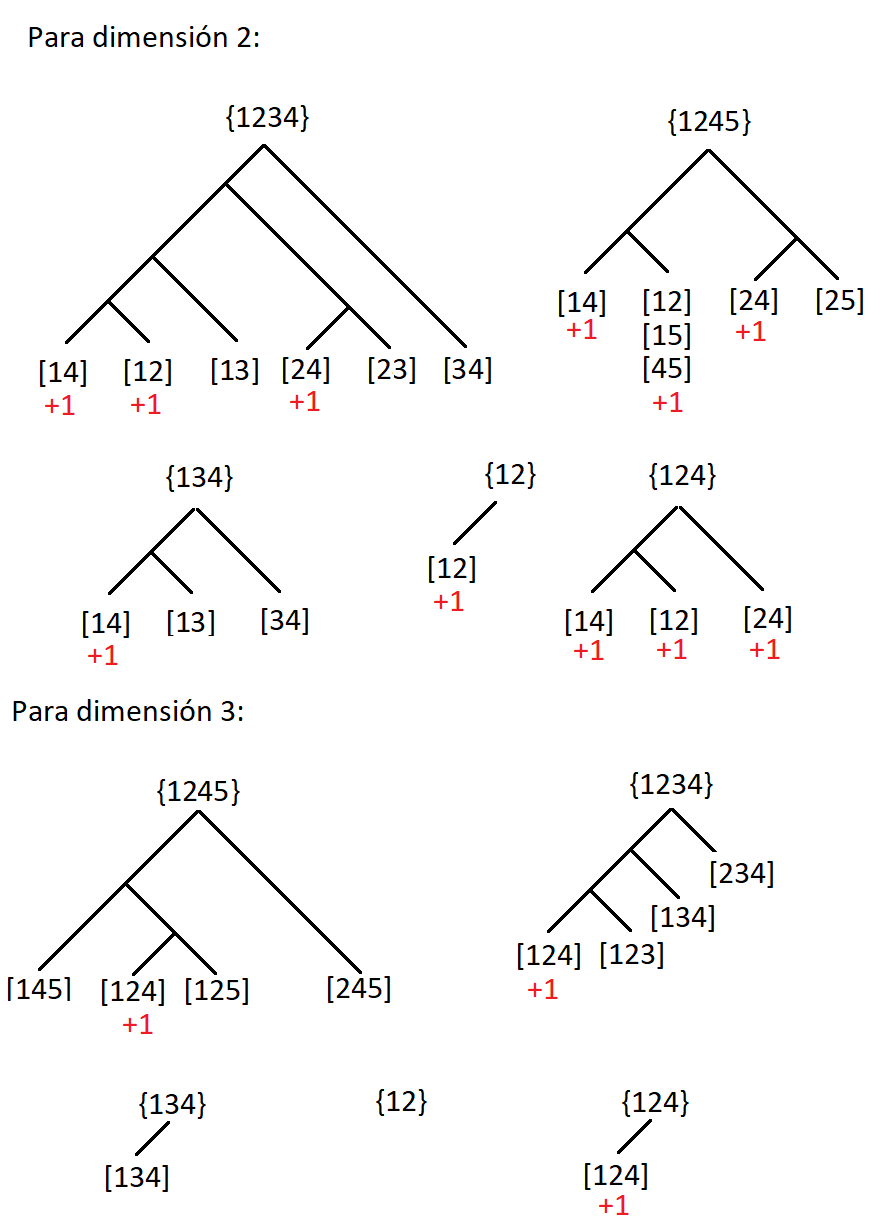
\includegraphics[width=0.8\linewidth]{images/apriori_muestras_2.png}
\caption{\label{fig:apriori_sucesos_muestra_2}Hash tree sucesos muestra con puntuación}
\end{figure}

\begin{figure}[H]
\centering
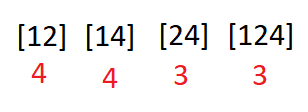
\includegraphics[width=0.8\linewidth]{images/apriori_candidatos_2.png}
\caption{\label{fig:apriori_sucesos_candidatos_2}Hash tree sucesos muestra con puntuación}
\end{figure}

Todos los sucesos llegan o superan el umbral de soporte (50\%).Por ejemplo, la confianza del suceso \{12\} es $\frac{n_{A_{i} \cup A_{j}}}{n_{T}}$ = $\frac{4}{6}$ = 66,67\% > 50\%.



Paso B: Se aplica únicamente a sucesos que llegan o superan el umbral de soporte. Se fija un umbral de confianza y se identifican las asociaciones que lo alcanzan o superan, y su sentido. Para cada suceso de dimensión k habrán $2^{k}-2$ posibles reglas de asociación

Para aquellos sucesos de tamaño 2, existen $2^{2}-2 = 2$ posibles asociaciones. Para aquellos sucesos de tamaño 3, existen $2^{3}-2 = 6$ posibles asociaciones.

Las posibles asociaciones de dimensión 2 son: 
\begin{enumerate}
    \item \{Pan\} -> \{Agua\}
    \item \{Agua\} -> \{Pan\}
    \item \{Pan\} -> \{Leche\}
    \item \{Leche\} -> \{Pan\}
    \item \{Agua\} -> \{Leche\}
    \item \{Leche\} -> \{Agua\}
\end{enumerate}

Todas las posibles asociaciones de dimensión 3 son: 
\begin{enumerate}
    \item \{Pan, Agua\} -> \{Leche\}
    \item \{Leche\} -> \{Pan, Agua\}
    \item \{Pan, Leche\} -> \{Agua\}
    \item \{Agua\} -> \{Pan, Leche\}
    \item \{Agua, Leche\} -> \{Pan\}
    \item \{Pan\} -> \{Agua, Leche\}
\end{enumerate}

Una vez determinado el número de asociaciones a considerar para cada suceso, dependiendo de su tamaño, se hacen dos pasos. El primero es aplicar gen-rules para establecer el umbral de confianza (en nuestro caso, utilizaremos el umbral c = 80\%). El último es paso es determinar las asociaciones que llegan o superan el umbral de confianza. Para ello nos ayudaremos del siguiente enunciado:

Sean A y B dos conjuntos, si se cumple que la asociación A -> B - A no supera el umbral de confianza, entonces podemos deducir que, siendo A' un subconjunto de A, todas las asociaciones A' -> B - A' tampoco alcanzarán ni superarán el umbral de confianza.

La confianza se expresa como: 

$\forall\{A_{i}\}_{i=1}^{\infty}\subset P(E) $ con $ A_{i} \cap A_{j} = \emptyset$ $\forall$ i != j, s:$P(E)$ ->  $ R+ / S(A_{i} \cup A_{j}) = \frac{n_{A_{i} \cup A_{j}}}{n_{A_{i}}}$

Empezamos por el suceso de mayor tamaño. Probamos con una de sus posibles asociaciones, por ejemplo, \{Pan, Agua\} -> \{Leche\}. Podemos identificar los conjuntos como $A_{i}$ = \{Pan, Agua\}, y $A_{j}$ = \{Leche\}. Una vez hecho, calculamos la confianza de este suceso:

c(\{Pan, Agua\} -> \{Leche\}) = $\frac{n_{A_{i} \cup A_{j}}}{A_{i}}$ = $\frac{3}{4}$ = 75\% < 80\%.

Ya que esta asociación no llega al umbral de confianza, podemos asegurar que tampoco lo harán las asociaciones \{Pan\} -> \{Agua, Leche\}, \{Agua\} -> \{Pan, Leche\}.

También podemos ir calculando las confianzas de los sucesos de tamaño 2:

c(\{Pan\} -> \{Agua\}) = $\frac{n_{A_{i} \cup A_{j}}}{A_{i}}$ = $\frac{4}{5}$ = 80\% = 80\%. -> Esta es una asociación solución
\newline
c(\{Leche\} -> \{Agua\}) = $\frac{n_{A_{i} \cup A_{j}}}{A_{i}}$ = $\frac{3}{4}$ = 75\% < 80\%. -> Esta asociación no llega al umbral de confianza.
...

Al final nos queda que, las asociaciones que superan el umbral de confianza son:

\begin{enumerate}
    \item \{Agua\} -> \{Pan\}
    \item \{Pan\} -> \{Agua\}
    \item \{Leche\} -> \{Pan\}
    \item \{Pan\} -> \{Leche\}
    \item \{Agua, Leche\} -> \{Pan\}
\end{enumerate}

En en paquete arules, existe la función apriori, a la cual podemos pasarle como argumentos la matriz  a priori que vamos a utilizar, el soporte y la confianza con la cual encontrar asociaciones, y nos devuelve las asociaciones que superan los umbrales de soporte y confianza.
Aplicamos ahora el algoritmo A Priori con los umbrales s >= 50\% y c >= 80\%, y mostramos el resultado por pantalla.


\begin{Schunk}
\begin{Sinput}
> asociaciones<-apriori(transacciones, parameter=list(support= 0.5, confidence= 0.8))
\end{Sinput}
\begin{Soutput}
Apriori

Parameter specification:
 confidence minval smax arem  aval originalSupport maxtime support minlen
        0.8    0.1    1 none FALSE            TRUE       5     0.5      1
 maxlen target  ext
     10  rules TRUE

Algorithmic control:
 filter tree heap memopt load sort verbose
    0.1 TRUE TRUE  FALSE TRUE    2    TRUE

Absolute minimum support count: 3 

set item appearances ...[0 item(s)] done [0.00s].
set transactions ...[5 item(s), 6 transaction(s)] done [0.00s].
sorting and recoding items ... [3 item(s)] done [0.00s].
creating transaction tree ... done [0.00s].
checking subsets of size 1 2 3 done [0.00s].
writing ... [7 rule(s)] done [0.00s].
creating S4 object  ... done [0.00s].
\end{Soutput}
\end{Schunk}


Para ver el resultado de ejecución, llamamos a la función inspect, que debería estar dentro del paquete de arules


\begin{Schunk}
\begin{Sinput}
> inspect(asociaciones)
\end{Sinput}
\begin{Soutput}
    lhs              rhs     support   confidence coverage  lift count
[1] {}            => {Leche} 0.8333333 0.8333333  1.0000000 1.00 5    
[2] {}            => {Pan}   0.8333333 0.8333333  1.0000000 1.00 5    
[3] {Agua}        => {Pan}   0.6666667 1.0000000  0.6666667 1.20 4    
[4] {Pan}         => {Agua}  0.6666667 0.8000000  0.8333333 1.20 4    
[5] {Leche}       => {Pan}   0.6666667 0.8000000  0.8333333 0.96 4    
[6] {Pan}         => {Leche} 0.6666667 0.8000000  0.8333333 0.96 4    
[7] {Agua, Leche} => {Pan}   0.5000000 1.0000000  0.5000000 1.20 3    
\end{Soutput}
\end{Schunk}


Tal y como se ha visto en clase de teoría, los resultados coinciden, siendo las asociaciones que superan ambos umbrales: 

\begin{enumerate}
    \item la 1
    \item la 2
    \item ...
\end{enumerate}

\subsection{Ejercicio 1.3}

En este apartado realizamos un ejercicio visto en clase de detección de outliers con técnicas estadísticas, en dos variables, Resistencia y Densidad, representados en la tabla novo\_muestra:


\begin{Schunk}
\begin{Sinput}
> novo_muestra <- data.frame(
+   Resistencia = c(3, 3.5, 4.7, 5.2, 7.1, 6.2, 14),
+   Densidad = c(2, 12, 4.1, 4.9, 6.1, 5.2, 5.3)
+ )
> (novo_muestra)
\end{Sinput}
\begin{Soutput}
  Resistencia Densidad
1         3.0      2.0
2         3.5     12.0
3         4.7      4.1
4         5.2      4.9
5         7.1      6.1
6         6.2      5.2
7        14.0      5.3
\end{Soutput}
\end{Schunk}


Primero empezamos con la técnica de Caja y Bigotes, para la variable Resistencia. Antes de comenzar, vamos a repasar los pasos del algoritmo a la vez que vamos resolviendo el ejercicio. Los pasos de la técnica de Caja y Bigotes son:

\begin{enumerate}
    \item Detección del grado de outlier. En nuestro caso, utilizaremos d = 1.5
    \item Se ordenan los datos y se obtienen los cuartiles. \nameref{fig:formula_cuartiles}
    \newline
    \newline
    Datos ordenados: 3, 3.5, 4.7, 5.2, 6.2, 7.1, 14
    \newline
    q1 = x$_{[7*0.25]+1}$ = x$_{2}$ = 3.5
    \newline
    q3 = x$_{[7*0.75]+1}$ = x$_{6}$ = 7.1
    \item Se calculan los límites del intervalo para los valores atípicos utilizando la ecuación: 
    ( q1 - d * (q3 - q1), q3 + d * (q3 - q1) )
    \newline
    \newline
    ( 3.5 - 1.5·(7.1-3.5), 7.1 + 1.5·(7.1-3.5) ) = ( -1.9, 12.5 )
    \item Se identifican los outliers como los valores que quedan fuera del intervalo, calculado en el paso 3.
    \newline
    \newline
    Para estos valores, identificamos que el valor de resistencia 14 es un outlier, ya que no se encuentra dentro del intervalo ( -1.9, 12.5 ).
\end{enumerate}

Ahora vamos a resolver el ejercicio con funciones en R:

Usando la función quantile calculamos el primer y tercer cuartil de la variable Resistencia.

\begin{Schunk}
\begin{Sinput}
> (cuar1r_resistencia <- quantile(novo_muestra$Resistencia, 0.25))
\end{Sinput}
\begin{Soutput}
25% 
4.1 
\end{Soutput}
\begin{Sinput}
> (cuar3r_resistencia <- quantile(novo_muestra$Resistencia, 0.75))
\end{Sinput}
\begin{Soutput}
 75% 
6.65 
\end{Soutput}
\end{Schunk}




Además, calculamos el rango intercuartil que define el intervalo para detectar valores atípicos.

\begin{Schunk}
\begin{Sinput}
> (int_resistencia <- c(
+ cuar1r_resistencia - 1.5 * (cuar3r_resistencia - cuar1r_resistencia), 
+ cuar3r_resistencia + 1.5 * (cuar3r_resistencia - cuar1r_resistencia)
+ ))
\end{Sinput}
\begin{Soutput}
   25%    75% 
 0.275 10.475 
\end{Soutput}
\end{Schunk}



Recorremos cada valor de la variable Resistencia y comprobamos si el valor está fuera del intervalo definido. Si el valor está fuera del intervalo definido, se imprime un mensaje.

\begin{Schunk}
\begin{Sinput}
> for (i in 1:length(novo_muestra$Resistencia)) {
+   if (novo_muestra$Resistencia[i] < int_resistencia[1] || 
+   novo_muestra$Resistencia[i] > int_resistencia[2]) {
+     print("El suceso")
+     print(i)
+     print(novo_muestra$Resistencia[i])
+     print("es un suceso anómalo u outlier en Resistencia")
+   }
+ }
\end{Sinput}
\begin{Soutput}
[1] "El suceso"
[1] 7
[1] 14
[1] "es un suceso anómalo u outlier en Resistencia"
\end{Soutput}
\end{Schunk}


La siguiente técnica que vamos a ver es aquella basada en métodos estadísticos utilizando la dispersión, y la vamos a utilizar para la variable Densidad. Los pasos de la técnica de métodos estadísticos son:

\begin{enumerate}
    \item Detección del grado de outlier. En nuestro caso, utilizaremos d = 2
    \item Se obtiene la media aritmética de los datos. \nameref{fig:formula_media_aritmetica}
    \newline
    \newline
    $\overline{x} = \frac{2+12+4.1+4.9+6.1+5.2+5.3}{7} = \frac{39,6}{7} = 5,66$    
    \item Se obtiene la desviación típica de los datos.
    \nameref{fig:formula_desviacion_tipica}
    \newline
    \newline
    $\sigma = \sqrt{\frac{(2-5,66)^{2}+(12-5,66)^{2}+...+(5.2-5,66)^{2}+(5.3-5,66)^{2}}{7}} = \sqrt{\frac{57,1372}{7}} = 2,86$
    \item Se calculan los límites del intervalo para los valores atípicos utilizando la ecuación: 
    ( $\overline{x}$ - d * $\sigma$, $\overline{x}$ + d * $\sigma$ )
    \newline
    \newline
    ( 5,66 - 2 · 2,86, 5,66 + 2 · 2,86 ) = ( -0,06, 11,38 )
    \item Se identifican los outliers como los valores que quedan fuera del intervalo, calculado en el paso 4.
    \newline
    \newline
    Para estos valores, identificamos que el valor de densidad 12 es un outlier, ya que no se encuentra dentro del intervalo ( -0,06, 11,38 ).
\end{enumerate}

Ahora vamos a resolver el ejercicio con funciones en R:




El primer paso es calcular la media y la desviación típica de la variable Densidad mediante las funciones mean y sdp.

\begin{Schunk}
\begin{Sinput}
> sdp <- function(x){ sqrt( (sd(x)^2) * ((length(x)-1)/length(x)) ) }
> (media_densidad <- mean(novo_muestra$Densidad))
\end{Sinput}
\begin{Soutput}
[1] 5.657143
\end{Soutput}
\begin{Sinput}
> (desviacion_densidad <- sdp(novo_muestra$Densidad))
\end{Sinput}
\begin{Soutput}
[1] 2.857
\end{Soutput}
\end{Schunk}




Se define un intervalo que se utilizará para la detección de valores atípicos en función de la media y la desviación estándar.

\begin{Schunk}
\begin{Sinput}
> (intdes_densidad <- c(
+ media_densidad - 2 * desviacion_densidad, 
+ media_densidad + 2 * desviacion_densidad
+ ))
\end{Sinput}
\begin{Soutput}
[1] -0.05685714 11.37114285
\end{Soutput}
\end{Schunk}




Se revisa cada valor de la variable Densidad y verifica si el valor está fuera del intervalo definido. Si el valor está fuera del intervalo, se imprime un mensaje.

\begin{Schunk}
\begin{Sinput}
> for (i in 1:length(novo_muestra$Densidad)) {
+   if (novo_muestra$Densidad[i] < intdes_densidad[1] || 
+   novo_muestra$Densidad[i] > intdes_densidad[2]) {
+     print("El suceso")
+     print(i)
+     print(novo_muestra$Densidad[i])
+     print("es un suceso anómalo o outlier en Densidad")
+   }
+ }
\end{Sinput}
\begin{Soutput}
[1] "El suceso"
[1] 2
[1] 12
[1] "es un suceso anómalo o outlier en Densidad"
\end{Soutput}
\end{Schunk}


Tal y como se ha visto en clase de teoría, los resultados coinciden.

\subsection{Ejercicio 1.4}

En este apartado realizamos un ejercicio visto en clase de detección de outliers con técnicas de proximidad (K vecinos) y densidad (LOF), en dos variables, Mujeres y Hombres, representados en la tabla muestra:


\begin{Schunk}
\begin{Sinput}
> muestra=matrix(c(4,4,4,3,5,5,1,1,5,4),2,5)
> (muestra)
\end{Sinput}
\begin{Soutput}
     [,1] [,2] [,3] [,4] [,5]
[1,]    4    4    5    1    5
[2,]    4    3    5    1    4
\end{Soutput}
\end{Schunk}


Es necesario trasponer esta matriz para empezar. Utilizaremos la función t() para ello:


\begin{Schunk}
\begin{Sinput}
> (muestra=t(muestra))
\end{Sinput}
\begin{Soutput}
     [,1] [,2]
[1,]    4    4
[2,]    4    3
[3,]    5    5
[4,]    1    1
[5,]    5    4
\end{Soutput}
\end{Schunk}


Antes de comenzar, vamos a repasar los pasos del algoritmo K vecinos, a la vez que vamos resolviendo el ejercicio. Los pasos del algoritmo K vecinos son:

Paso A: 

\begin{enumerate}
    \item Determinación del grado de outlier, el cual es la distancia con la cual el suceso (punto) empieza a considerarse un outlier. En nuestro caso, establecemos d = 2,5.
    \item Determinación del número de orden, o K, del vecino más próximo para el que el suceso sea considerado un outlier. En nuestro caso, establecemos K = 3
\end{enumerate}

Paso B:

%(4,4) (4,3) (5,5) (1,1) (5,4)

\begin{enumerate}
    \item Cálculo de las distancias euclídeas entre todos los puntos. la distancia se define como distancia($x_{i}$, $x_{j}$) = $\sqrt{(x_{i1}-x_{j1})^{2} + (x_{i2}-x_{j2})^{2}}$
    \newline
    \newline
    distancia(1,2) = $\sqrt{(x_{i1}-x_{j1})^{2} + (x_{i2}-x_{j2})^{2}}$ = $\sqrt{(4-4)^{2} + (4-3)^{2}}$ = 1
    \newline
    distancia(1,3) = $\sqrt{(4-5)^{2} + (4-5)^{2}}$ = 1.41
    \newline
    distancia(1,4) = $\sqrt{(4-1)^{2} + (4-1)^{2}}$ = 4.24
    \newline
    distancia(1,5) = $\sqrt{(4-5)^{2} + (4-4)^{2}}$ = 1
    \newline
    distancia(2,3) = $\sqrt{(4-5)^{2} + (3-5)^{2}}$ = 2.24
    \newline
    distancia(2,4) = $\sqrt{(4-1)^{2} + (3-1)^{2}}$ = 3.61
    \newline
    distancia(2,5) = $\sqrt{(4-5)^{2} + (3-4)^{2}}$ = 1.41
    \newline
    distancia(3,4) = $\sqrt{(5-1)^{2} + (5-1)^{2}}$ = 5.66
    \newline
    distancia(3,5) = $\sqrt{(5-5)^{2} + (5-4)^{2}}$ = 1
    \newline
    distancia(4,5) = $\sqrt{(1-5)^{2} + (1-4)^{2}}$ = 5
    \item Ordenación por distancias de los vecinos de cada punto hasta llegar al K definido
    \newline
    \newline
    \begin{center}
    \begin{tabular}{ |p{3cm}||p{3cm}|p{3cm}|p{3cm}|  }
    \hline
    \multicolumn{4}{|c|}{Distancias ordenadas por K} \\
    \hline
    Punto \textbackslash K& K = 1 &K = 2&K = 3\\
    \hline
    P(1)&   P(2)=1   &  P(5)=1   &  P(3)=1.41\\
    P(2)&   P(1)=1   &  P(5)=1.41   &  P(3)=2.24\\
    P(3)&   P(5)=1   &  P(1)=1.41   &  P(2)=2.24\\
    P(4)&   P(2)=3.61&  P(1)=4.24&  P(5)=5\\
    P(5)&   P(1)=1   &  P(3)=1   &  P(2)=1.41\\
    \hline
    \end{tabular}
    \end{center}
    \item Identificación de los outliers como aquellos sucesos cuyo K vecino se encuentre a una distancia mayor que el grado de outlier definido
    \newline
    \newline
    Podemos observar que el único punto cuya distancia al vecino K = 3 más próximo mayor que el grado de outlier es el punto 4 (1,1). Por tanto, este punto es considerado un outlier.
\end{enumerate}

Ahora vamos a resolver el ejercicio con funciones en R:

Vamos a utilizar el mismo grado de outlier d = 2,5 y el número de orden K = 4, debido a que R tiene en cuenta la distancia del punto consigo mismo que siempre es 0, lo que hace que sea el vecino más próximo a cada punto. 



Lo siguiente es calcular, para cada punto, la distancia a la que está con respecto al resto de puntos. Para ello, vamos a utilizar la función  dist(), y vamos a cambiar el tipo del resultado con la función as.matrix():


\begin{Schunk}
\begin{Sinput}
> (distancias=as.matrix(dist(muestra)))
\end{Sinput}
\begin{Soutput}
         1        2        3        4        5
1 0.000000 1.000000 1.414214 4.242641 1.000000
2 1.000000 0.000000 2.236068 3.605551 1.414214
3 1.414214 2.236068 0.000000 5.656854 1.000000
4 4.242641 3.605551 5.656854 0.000000 5.000000
5 1.000000 1.414214 1.000000 5.000000 0.000000
\end{Soutput}
\end{Schunk}




Ahora ordenaremos las distancias de menor a mayor. Para ello, primero vamos a definir el resultado de antes como una matrix, de tantas filas y columnas como K+1:


\begin{Schunk}
\begin{Sinput}
> (distancias=matrix(distancias,5,5))
\end{Sinput}
\begin{Soutput}
         [,1]     [,2]     [,3]     [,4]     [,5]
[1,] 0.000000 1.000000 1.414214 4.242641 1.000000
[2,] 1.000000 0.000000 2.236068 3.605551 1.414214
[3,] 1.414214 2.236068 0.000000 5.656854 1.000000
[4,] 4.242641 3.605551 5.656854 0.000000 5.000000
[5,] 1.000000 1.414214 1.000000 5.000000 0.000000
\end{Soutput}
\end{Schunk}




Ahora si que hacemos la ordenación de las distancias. Recorreremos con un bucle for todas las columnas de la matriz, y ordenaremos sus valores de puntos de menor a mayor:


\begin{Schunk}
\begin{Sinput}
> for (i in 1:5) { 
+ distancias[,i] = sort(distancias[,i]) }; 
> ( distanciasordenadas = distancias )
\end{Sinput}
\begin{Soutput}
         [,1]     [,2]     [,3]     [,4]     [,5]
[1,] 0.000000 0.000000 0.000000 0.000000 0.000000
[2,] 1.000000 1.000000 1.000000 3.605551 1.000000
[3,] 1.000000 1.414214 1.414214 4.242641 1.000000
[4,] 1.414214 2.236068 2.236068 5.000000 1.414214
[5,] 4.242641 3.605551 5.656854 5.656854 5.000000
\end{Soutput}
\end{Schunk}


Por último, recorremos, para cada columna, la fila K = 4, y para cada punto de dicho orden, observamos si su distancia supera el grado de outlier. En el caso de que se cumpla dicha condición, podemos concluir que, el punto en la columna actual es un outlier. Para ello, utilizamos el siguiente código:


\begin{Schunk}
\begin{Sinput}
> for (i in 1:5) { if(distanciasordenadas[4,i] > 2.5 ) {
+ print(i); print("Es un suceso anómalo o outlier") 
+ } }
\end{Sinput}
\begin{Soutput}
[1] 4
[1] "Es un suceso anómalo o outlier"
\end{Soutput}
\end{Schunk}


Tal y como se ha visto en clase de teoría, los resultados coinciden.

Esta última función se puede llegar a acortar, para juntar los dos últimos pasos en uno:


\begin{Schunk}
\begin{Sinput}
> for (i in 1:5) { distancias[,i]=sort(distancias[,i])
+ if (distancias[4,i] > 2.5) { print(i)
+ print("Es un suceso anómalo o outlier")
+ }
+ }
\end{Sinput}
\begin{Soutput}
[1] 4
[1] "Es un suceso anómalo o outlier"
\end{Soutput}
\end{Schunk}


Ahora vamos a encontrar outliers pero con la técnica de densidades LOF. Antes de comenzar, vamos a repasar los pasos del algoritmo LOF, a la vez que vamos resolviendo el ejercicio. Los pasos del algoritmo LOF son:

Paso A: Determinación del grado de outlier (en nuestro caso, d = 2.5), definiendo la densidad en cada punto, definida como:

densidad($x_{i}$,K) = ${(\frac{\Sigma _{x_{i} \in N(x_{i}, K)}distancia(x_{i}, x_{j})}{cardinal N(x_{i},K)}})^{-1}$

Este paso está dividido en 4 subpasos:

%(4,4) (4,3) (5,5) (1,1) (5,4)

\begin{enumerate}
    \item Determinación del número de orden K (en nuestro caso, K = 3)
    \item Cálculo de las distancias Manhattan entre todos los puntos. la distancia se define como distancia($x_{i}$, $x_{j}$) = $|x_{i1}-x_{j1}| + |x_{i2}-x_{j2}|$ 
    \newline
    \newline
    distancia(1,2) = $|x_{i1}-x_{j1}| + |x_{i2}-x_{j2}|$ = $|4-4| + |4-3|$ = 1
    \newline
    distancia(1,3) = $|4-5| + |4-5|$ = 2
    \newline
    distancia(1,4) = $|4-1| + |4-1|$ = 6
    \newline
    distancia(1,5) = $|4-5| + |4-4|$ = 1
    \newline
    distancia(2,3) = $|4-5| + |3-5|$ = 3
    \newline
    distancia(2,4) = $|4-1| + |3-1|$ = 5
    \newline
    distancia(2,5) = $|4-5| + |3-4|$ = 2
    \newline
    distancia(3,4) = $|5-1| + |5-1|$ = 8
    \newline
    distancia(3,5) = $|5-5| + |5-4|$ = 1
    \newline
    distancia(4,5) = $|1-5| + |1-4|$ = 7
    \item Cálculo del cardinal o tamaño del conjunto N para cada punto. N es el conjunto que contiene los vecinos cuya distancia a $x_{i}$ es igual o inferior a la K del vecino más próximo
    \newline
    \newline
    \begin{center}
    \begin{tabular}{ |p{2cm}||p{2cm}|p{2cm}|p{2cm}|p{2cm}|  }
    \hline
    \multicolumn{5}{|c|}{Distancias ordenadas por K} \\
    \hline
    Punto \textbackslash K& K = 1 &K = 2&K = 3&N\\
    \hline
    P(1)&   P(2)=1   &  P(5)=1   &  P(3)=2  &   N=3\\
    P(2)&   P(1)=1   &  P(5)=2   &  P(3)=3  &   N=3\\
    P(3)&   P(5)=1   &  P(1)=2   &  P(2)=3  &   N=3\\
    P(4)&   P(2)=5   &  P(1)=6   &  P(5)=7  &   N=3\\
    P(5)&   P(1)=1   &  P(3)=1   &  P(2)=2  &   N=3\\
    \hline
    \end{tabular}
    \end{center}

    \item Cálculo de la densidad de cada punto, utilizando los datos de los dos pasos anteriores, con la expresión vista en el paso A
    \newline
    densidad(1,K) = ${(\frac{\Sigma _{x_{i} \in N(x_{i}, K)}distancia(x_{i}, x_{j})}{cardinal N(x_{i},K)}})^{-1}$ = ${(\frac{distancia(1, 2)+distancia(1, 5)+distancia(1, 3)}{cardinal N(1,K)}})^{-1}$ = $\frac{3}{1+1+2}$ = 0.75
    \newline
    densidad(2,K) = $\frac{3}{1+2+3}$ = 0.5
    \newline
    densidad(3,K) = $\frac{3}{1+2+3}$ = 0.5
    \newline
    densidad(4,K) = $\frac{3}{5+6+7}$ = 0.17
    \newline
    densidad(5,K) = $\frac{3}{1+1+2}$ = 0.75
\end{enumerate}

Paso B: Cálculo de la densidad relativa media de cada punto (drm). La expresión de la densidad media relativa es:

densidad relativa media($x_i$,K) = $\frac{densidad(x_{i},K)}{\frac{\Sigma _{x_{j} \in N(x_{i}, K)}densidad(x_{j}, K)}{cardinal N(x_{i},K)}}$
\newline
drm(1,K) = $\frac{densidad(x_{i},K)}{\frac{\Sigma _{x_{j} \in N(x_{i}, K)}densidad(x_{j}, K)}{cardinal N(x_{i},K)}}$ = $\frac{densidad(1,K)}{\frac{densidad(2,K)+densidad(5,K)+distancia(3,K)}{cardinal N(1,K)}}$ = $\frac{0.75}{\frac{0.5+0.5+0.75}{3}}$ = 1.29
\newline
drm(2,K) = $\frac{0.5}{\frac{0.5+0.5+0.75}{3}}$ = 0.75
\newline
drm(3,K) = $\frac{0.5}{\frac{0.5+0.5+0.75}{3}}$ = 0.75
\newline
drm(4,K) = $\frac{0.17}{\frac{0.75+0.5+0.75}{3}}$ = 0.26
\newline
drm(5,K) = $\frac{0.75}{\frac{0.5+0.5+0.75}{3}}$ = 1.29

Paso C: Obtención de los outliers, como aquellos puntos cuya densidad relativa sea significativamente menor que la del resto de elementos de la muestra. Se pueden establecer diferentes métodos para establecer cuándo la drm es significativamente menor. En nuestro caso, tomaremos como outlier el punto con menor valor de densidad relativa media.

Podríamos escoger una métrica más elaborada, pero vamos a considerar outlier a aquel punto con la drm más baja. En este caso, el outlier es el punto 4.

Ahora resolveríamos el ejercicio con funciones en R, pero únicamente vamos a hacer el paso A, hasta su subpaso 2:

El grado de outlier sería d = 2,5 y el número de orden K = 4.

Al igual que en K vecinos, cargamos la tabla y calculamos las distancias, aunque ahora son distancias Manhattan:


\begin{Schunk}
\begin{Sinput}
> muestra=matrix(c(4,4,4,3,5,5,1,1,5,4),2,5)
> (muestra)
\end{Sinput}
\begin{Soutput}
     [,1] [,2] [,3] [,4] [,5]
[1,]    4    4    5    1    5
[2,]    4    3    5    1    4
\end{Soutput}
\begin{Sinput}
> (muestra=t(muestra))
\end{Sinput}
\begin{Soutput}
     [,1] [,2]
[1,]    4    4
[2,]    4    3
[3,]    5    5
[4,]    1    1
[5,]    5    4
\end{Soutput}
\begin{Sinput}
> (distancias=as.matrix(dist(muestra, method="manhattan")))
\end{Sinput}
\begin{Soutput}
  1 2 3 4 5
1 0 1 2 6 1
2 1 0 3 5 2
3 2 3 0 8 1
4 6 5 8 0 7
5 1 2 1 7 0
\end{Soutput}
\end{Schunk}


Ahora tendríamos que continuar con los pasos que hemos visto del algoritmo para terminar el ejercicio. 

Podemos encontrar en el archivo CRAN algunos paquetes como \href{https://cran.r-project.org/web/packages/Rlof/index.html}{Rlof} y \href{https://cran.r-project.org/web/packages/Rlof/index.html}{DDoutlier}, que tienen una implementación del LOF, pero con unos pasos distintos a lo visto en clase.

Ambas implementaciones se basan en el algoritmo propuesto en \href{https://dl.acm.org/doi/pdf/10.1145/335191.335388}{este artículo}.

\section{Parte 2}

En esta parte, vamos a repetir los ejercicios anteriores, pero utilizaremos datos diferentes y propondremos una forma de solucionarlos distinta a la vista en clase.

\subsection{Ejercicio 2.1}

Lo primero que vamos a hacer es cargar la tabla con los datos necesarios para hacer el análisis estadístico. Para ello, llamamos a las siguientes funciones:


\begin{Schunk}
\begin{Sinput}
> distancias<-c(16.5, 34.8, 20.7, 6.2, 4.4, 3.4, 24, 24, 32, 30, 33, 27, 
+ 15, 9.4, 2.1, 34, 24, 12, 4.4, 28, 31.4, 21.6, 3.1, 4.5, 5.1, 4, 3.2,
+ 25, 4.5, 20, 34, 12, 12, 12, 12, 5, 19, 30, 5.5, 38, 25, 3.7, 9, 30,
+ 13, 30, 30, 26, 30, 30, 1, 26, 22, 10, 9.7, 11, 24.1, 33, 17.2,
+ 27, 24, 27, 21, 28, 30, 4, 46, 29, 3.7, 2.7, 8.1, 19, 16)
\end{Sinput}
\end{Schunk}


Se han implementado las siguientes funciones auxiliares para implementar el resto de funciones matemáticas:

\begin{enumerate}

\item 

\begin{Schunk}
\begin{Sinput}
> calcular_absoluto <-
+ function(dato){
+     if (dato < 0){
+         return (-dato)
+     }else{
+         return(dato)
+     }
+ }
> calcular_absoluto(-3)
\end{Sinput}
\begin{Soutput}
[1] 3
\end{Soutput}
\begin{Sinput}
> calcular_absoluto(3)
\end{Sinput}
\begin{Soutput}
[1] 3
\end{Soutput}
\end{Schunk}

La función calcular\_absoluto devuelve un valor pasado como argumento si su signo es positivo, o el negado de dicho número si su signo es negativo

\item 

\begin{Schunk}
\begin{Sinput}
> longitud <- 
+ function (datos){
+     contador <- 0
+     for (elemento in datos){
+         contador <- contador + 1
+     }
+     return (contador)
+ }
> longitud(distancias)
\end{Sinput}
\begin{Soutput}
[1] 73
\end{Soutput}
\end{Schunk}

La función longitud devuelve la longitud de una lista pasada como argumento. Se inicializa una variable con valor a 0. Se recorren los elementos de la lista, y para cada iteración, se incrementa el valor del contador en 1. Finalmente, se devuelve el contador

\item 

\begin{Schunk}
\begin{Sinput}
> contar <- 
+ function(conjunto,elemento){
+     contador <- 0
+     for (i in conjunto){
+         if (i == elemento){
+             contador <- contador + 1
+         }
+     }
+     return (contador)
+ }
> contar(distancias,30)
\end{Sinput}
\begin{Soutput}
[1] 8
\end{Soutput}
\end{Schunk}

La función contar devuelve el número de veces que un elemento pertenece a un conjunto, representado como una lista. Se inicializa una variable con valor a 0. Se recorren los elementos de la lista, y para cada iteración, se incrementa el valor del contador en 1 si el elemento pasado como argumento es igual que el elemento en la posición actual de la iteración. Finalmente, se devuelve el contador.

\item 

\begin{Schunk}
\begin{Sinput}
> calcular_maximo <-
+ function(datos){
+     mayor <- 0
+     for (i in 1:longitud(datos)){
+         if (datos[[i]] > mayor){
+             mayor <- datos[[i]]
+         }
+     }
+     return (mayor)
+ }
> calcular_maximo(distancias)
\end{Sinput}
\begin{Soutput}
[1] 46
\end{Soutput}
\end{Schunk}

Devuelve el elemento de mayor valor de una lista pasada como argumento. Primero se establece el valor de una variable temporal mayor a 0. Después se va recorriendo la lista pasada como argumento. Para cada valor, si llega a ser mayor que el actual valor de mayor, entonces el valor de la variable mayor pasa a ser el valor del elemento en la iteración actual. Finalmente, se devuelve el valor de la variable mayor

\item 

\begin{Schunk}
\begin{Sinput}
> ordenar_burbuja <-
+ function(vector) {
+   n <- longitud(vector)
+   for (i in 1:(n - 1)) {
+     for (j in 1:(n - i)) {
+       if (vector[j] > vector[j + 1]) {
+         # Intercambiar elementos si están en el orden incorrecto
+         temp <- vector[j]
+         vector[j] <- vector[j + 1]
+         vector[j + 1] <- temp
+       }
+     }
+   }
+   return(vector)
+ }
> ordenar_burbuja(distancias)
\end{Sinput}
\begin{Soutput}
 [1]  1.0  2.1  2.7  3.1  3.2  3.4  3.7  3.7  4.0  4.0  4.4  4.4  4.5  4.5  5.0
[16]  5.1  5.5  6.2  8.1  9.0  9.4  9.7 10.0 11.0 12.0 12.0 12.0 12.0 12.0 13.0
[31] 15.0 16.0 16.5 17.2 19.0 19.0 20.0 20.7 21.0 21.6 22.0 24.0 24.0 24.0 24.0
[46] 24.1 25.0 25.0 26.0 26.0 27.0 27.0 27.0 28.0 28.0 29.0 30.0 30.0 30.0 30.0
[61] 30.0 30.0 30.0 30.0 31.4 32.0 33.0 33.0 34.0 34.0 34.8 38.0 46.0
\end{Soutput}
\end{Schunk}

La función ordenar toma una lista de elementos, preferiblemente números, y devuelve una lista con dichos elementos ordenados ascendentemente. Para ordenar los elementos, se utiliza el algoritmo de ordenación de la burbuja, en el cual se van recorriendo las posiciones de la lista n veces, cada iteración recorriendo i-n elementos, siendo i el número de la iteración actual. En cada vez que se pasa por la lista, se comprueba en la posición actual si el elemento posterior a la iteración actual está desordenado, y en ese caso se cambia su orden. Al terminar el algoritmo, la función devuelve la lista de elementos ordenados

\end{enumerate}

Vamos a empezar con la primera parte del análisis de los datos. Para obtener las frecuencias, se han implementado las siguientes funciones:

\begin{enumerate}

\item

\begin{Schunk}
\begin{Sinput}
> calcular_frecuencia_absoluta <- 
+ function(datos) {
+     valores <- unique(datos)
+     frecuencias <- numeric(longitud(valores))
+     for (elemento in 1:longitud(valores)){
+         frecuencias[elemento] <- contar(datos,valores[elemento])
+     }
+     frecuencia_absoluta<-data.frame(distancia = valores, frecuencia = frecuencias)
+     return (frecuencia_absoluta)
+ }
\end{Sinput}
\end{Schunk}

La función calcular\_frecuencia\_absoluta() devuelve una tabla con tantas filas como valores diferentes se encuentren en una lista pasada como argumentos, y dos columnas, en la primera con los valores diferentes, y en la segunda con el número de veces que se repite dicho valor en la lista. Primero se crea una lista con los elementos únicos con unique(). Después se recorre la lista pasada como argumento, y se asigna a una lista con las frecuencias el resultado de llamar a la función contar en la lista pasada como argumento el elemento actualmente recorrido en la iteración. Posteriormente se crea un data.frame cuya primera columna son los valores únicos, y la segunda los valores de frecuencias de cada uno. Finalmente se devuelve la tabla resultado valor diferente de la lista pasada como argumento, y en la segunda columna, el número de veces que se repite dicho valor.
Vamos a calcular las frecuencias absolutas de los datos del ejercicio:

\begin{Schunk}
\begin{Sinput}
> calcular_frecuencia_absoluta(distancias)
\end{Sinput}
\begin{Soutput}
   distancia frecuencia
1       16.5          1
2       34.8          1
3       20.7          1
4        6.2          1
5        4.4          2
6        3.4          1
7       24.0          4
8       32.0          1
9       30.0          8
10      33.0          2
11      27.0          3
12      15.0          1
13       9.4          1
14       2.1          1
15      34.0          2
16      12.0          5
17      28.0          2
18      31.4          1
19      21.6          1
20       3.1          1
21       4.5          2
22       5.1          1
23       4.0          2
24       3.2          1
25      25.0          2
26      20.0          1
27       5.0          1
28      19.0          2
29       5.5          1
30      38.0          1
31       3.7          2
32       9.0          1
33      13.0          1
34      26.0          2
35       1.0          1
36      22.0          1
37      10.0          1
38       9.7          1
39      11.0          1
40      24.1          1
41      17.2          1
42      21.0          1
43      46.0          1
44      29.0          1
45       2.7          1
46       8.1          1
47      16.0          1
\end{Soutput}
\end{Schunk}


\item

\begin{Schunk}
\begin{Sinput}
> calcular_frecuencia_relativa <- 
+ function(datos) {
+     valores <- unique(datos)
+     frecuencias <- numeric(longitud(valores))
+     for (elemento in 1:longitud(valores)){
+         frecuencias[elemento] <- contar(datos,valores[elemento])
+     }
+     frecuencia_relativa<-data.frame(distancia = valores, frecuencia = frecuencias/longitud(datos))
+     return (frecuencia_relativa)
+ }
\end{Sinput}
\end{Schunk}

La función calcular\_frecuencia\_relativa() devuelve una tabla con tantas filas como valores diferentes se encuentren en una lista pasada como argumentos, y dos columnas, en la primera con los valores diferentes, y en la segunda con el número de veces que se repite dicho valor en la lista, dividido entre el total de elementos que tiene la lista. Funciona igual que la función calcular\_frecuencia\_absoluta, pero al final, al crear el data.frame, se divide cada valor de la lista frecuencias entre el número de elementos de la lista.
Vamos a calcular las frecuencias relativas de los datos del ejercicio:

\begin{Schunk}
\begin{Sinput}
> calcular_frecuencia_relativa(distancias)
\end{Sinput}
\begin{Soutput}
   distancia frecuencia
1       16.5 0.01369863
2       34.8 0.01369863
3       20.7 0.01369863
4        6.2 0.01369863
5        4.4 0.02739726
6        3.4 0.01369863
7       24.0 0.05479452
8       32.0 0.01369863
9       30.0 0.10958904
10      33.0 0.02739726
11      27.0 0.04109589
12      15.0 0.01369863
13       9.4 0.01369863
14       2.1 0.01369863
15      34.0 0.02739726
16      12.0 0.06849315
17      28.0 0.02739726
18      31.4 0.01369863
19      21.6 0.01369863
20       3.1 0.01369863
21       4.5 0.02739726
22       5.1 0.01369863
23       4.0 0.02739726
24       3.2 0.01369863
25      25.0 0.02739726
26      20.0 0.01369863
27       5.0 0.01369863
28      19.0 0.02739726
29       5.5 0.01369863
30      38.0 0.01369863
31       3.7 0.02739726
32       9.0 0.01369863
33      13.0 0.01369863
34      26.0 0.02739726
35       1.0 0.01369863
36      22.0 0.01369863
37      10.0 0.01369863
38       9.7 0.01369863
39      11.0 0.01369863
40      24.1 0.01369863
41      17.2 0.01369863
42      21.0 0.01369863
43      46.0 0.01369863
44      29.0 0.01369863
45       2.7 0.01369863
46       8.1 0.01369863
47      16.0 0.01369863
\end{Soutput}
\end{Schunk}


\item

\begin{Schunk}
\begin{Sinput}
> calcular_frecuencia_absoluta_acumulada <-
+ function(datos) {
+     valores <- unique(ordenar_burbuja(datos))
+     frecuencias <- numeric(longitud(valores))
+     frec_abs_acum <- numeric(longitud(valores))
+     for (elemento in 1:longitud(valores)){
+         frecuencias[elemento] <- contar(datos,valores[elemento])
+     }
+     frec_abs_acum[1] <- frecuencias[1]
+     for (i in 2:longitud(valores)){
+         frec_abs_acum[i] <- (frecuencias[i]+frec_abs_acum[i-1])
+     }
+     frecuencia_absoluta_acum<-data.frame(distancia = valores, frecuencia = frec_abs_acum)
+     return (frecuencia_absoluta_acum)
+ }
\end{Sinput}
\end{Schunk}

La función calcular\_frecuencia\_absoluta\_acumulada() devuelve una tabla con tantas filas como valores diferentes se encuentren en una lista pasada como argumentos, y dos columnas, en la primera con los valores diferentes, y en la segunda con el valor de la frecuencia absoluta acumulada de dicho valor, siendo la frecuencia absoluta acumulada del último valor igual que el número de elementos de la lista. Primero se toman los valores únicos de la lista, y también se ordenan de menor a mayor. Después se recorre la lista y se llama a la función contar al igual que en calcular\_frecuencia\_absoluta. Lo siguiente que se hace es recorrer la lista desde el segundo elemento hasta el final, incrementando el valor actual de la iteración con el valor de frecuencia del valor en la posición de la iteración anterior. Finalmente, se vuelve a generar el mismo data.frame generado en calcular\_frecuencia\_absoluta, pero con las frecuencias absolutas acumuladas
Vamos a calcular las frecuencias absolutas acumuladas de los datos del ejercicio:

\begin{Schunk}
\begin{Sinput}
> calcular_frecuencia_absoluta_acumulada(distancias)
\end{Sinput}
\begin{Soutput}
   distancia frecuencia
1        1.0          1
2        2.1          2
3        2.7          3
4        3.1          4
5        3.2          5
6        3.4          6
7        3.7          8
8        4.0         10
9        4.4         12
10       4.5         14
11       5.0         15
12       5.1         16
13       5.5         17
14       6.2         18
15       8.1         19
16       9.0         20
17       9.4         21
18       9.7         22
19      10.0         23
20      11.0         24
21      12.0         29
22      13.0         30
23      15.0         31
24      16.0         32
25      16.5         33
26      17.2         34
27      19.0         36
28      20.0         37
29      20.7         38
30      21.0         39
31      21.6         40
32      22.0         41
33      24.0         45
34      24.1         46
35      25.0         48
36      26.0         50
37      27.0         53
38      28.0         55
39      29.0         56
40      30.0         64
41      31.4         65
42      32.0         66
43      33.0         68
44      34.0         70
45      34.8         71
46      38.0         72
47      46.0         73
\end{Soutput}
\end{Schunk}


\item

\begin{Schunk}
\begin{Sinput}
> calcular_frecuencia_relativa_acumulada <- 
+ function(datos) {
+     valores <- unique(ordenar_burbuja(datos))
+     frecuencias <- numeric(longitud(valores))
+     frec_rel_acum <- numeric(longitud(valores))
+     for (elemento in 1:longitud(valores)){
+         frecuencias[elemento] <- contar(datos,valores[elemento])
+     }
+     frecuencias_relativas<-frecuencias/longitud(datos)
+     frec_rel_acum[1]<-frecuencias_relativas[1]
+     for (i in 2:longitud(valores)){
+         frec_rel_acum[i] <- (frecuencias_relativas[i]+frec_rel_acum[i-1])
+     }
+     frecuencia_relativa_acum<-data.frame(distancia = valores, frecuencia = frec_rel_acum)
+     return (frecuencia_relativa_acum)
+ }
\end{Sinput}
\end{Schunk}

La función calcular\_frecuencia\_absoluta\_acumulada devuelve una tabla con tantas filas como valores diferentes se encuentren en una lista pasada como argumentos, y dos columnas, en la primera con los valores diferentes, y en la segunda con el valor de la frecuencia relativa acumulada de dicho valor, siendo la frecuencia relativa acumulada del último valor igual a 1. Se lleva a cabo el mismo procedimiento que en calcular\_frecuencia\_absoluta\_acumulada, pero la diferencia está en que, antes de ir calculando el sumatorio, recorriendo la lista de frecuencias. Se dividen todos los valores de frecuencias absolutas entre el número de elementos de la lista argumento.
Vamos a calcular las frecuencias relativas acumuladas de los datos del ejercicio:

\begin{Schunk}
\begin{Sinput}
> calcular_frecuencia_relativa_acumulada(distancias)
\end{Sinput}
\begin{Soutput}
   distancia frecuencia
1        1.0 0.01369863
2        2.1 0.02739726
3        2.7 0.04109589
4        3.1 0.05479452
5        3.2 0.06849315
6        3.4 0.08219178
7        3.7 0.10958904
8        4.0 0.13698630
9        4.4 0.16438356
10       4.5 0.19178082
11       5.0 0.20547945
12       5.1 0.21917808
13       5.5 0.23287671
14       6.2 0.24657534
15       8.1 0.26027397
16       9.0 0.27397260
17       9.4 0.28767123
18       9.7 0.30136986
19      10.0 0.31506849
20      11.0 0.32876712
21      12.0 0.39726027
22      13.0 0.41095890
23      15.0 0.42465753
24      16.0 0.43835616
25      16.5 0.45205479
26      17.2 0.46575342
27      19.0 0.49315068
28      20.0 0.50684932
29      20.7 0.52054795
30      21.0 0.53424658
31      21.6 0.54794521
32      22.0 0.56164384
33      24.0 0.61643836
34      24.1 0.63013699
35      25.0 0.65753425
36      26.0 0.68493151
37      27.0 0.72602740
38      28.0 0.75342466
39      29.0 0.76712329
40      30.0 0.87671233
41      31.4 0.89041096
42      32.0 0.90410959
43      33.0 0.93150685
44      34.0 0.95890411
45      34.8 0.97260274
46      38.0 0.98630137
47      46.0 1.00000000
\end{Soutput}
\end{Schunk}


\end{enumerate}

Ahora vamos a realizar la segunda parte del análisis de datos:

\begin{enumerate}

\item 

\begin{Schunk}
\begin{Sinput}
> calcular_moda <- 
+ function(datos){
+     frecuencias <- calcular_frecuencia_absoluta(datos)
+     maximo <- calcular_maximo(frecuencias[2][[1]])
+     moda <- frecuencias[1][frecuencias[2] == maximo]
+     return (moda)
+ }
\end{Sinput}
\end{Schunk}

la función calcular\_moda() devuelve el valor de la moda de una lista pasada como argumento. Primero se llama a la función calcular\_frecuencia\_absoluta pasando como argumento, la lista que hemos pasado a esta función de moda. Después obtenemos el valor máximo de frecuencia de la columna de frecuencias obtenidas de calcular\_frecuencia\_absoluta, con la función calcular\_maximo. Finalmente, tomamos el valor de la moda como aquel que en la tabla obtenida con calcular\_frecuencia\_absoluta cumpla que su frecuencia absoluta sea igual que el valor máximo que determinamos anteriormente, y devolvemos dicho valor.
Al llamar a esta función, obtenemos que la moda de los datos es:

\begin{Schunk}
\begin{Sinput}
> calcular_moda(distancias)
\end{Sinput}
\begin{Soutput}
[1] 30
\end{Soutput}
\end{Schunk}



\begin{Schunk}
\begin{Sinput}
> calcular_media <- 
+ function(datos){
+     media <- 0
+     for (i in 1:longitud(datos)){
+         media <- media + datos[i]
+     }
+     media <- media/longitud(datos)
+     return (media)
+ }
\end{Sinput}
\end{Schunk}

La función calcular\_media devuelve la media aritmética de una lista pasada como argumento. Primero se inicia una variable temporal a 0. Después se van recorriendo los elementos de la lista, e incrementando el valor de la variable temporal por el valor del elemento actual en la iteración. Una vez se han recorrido todos los elementos, se divide este valor entre el resultado que devuelve la llamada a la función longitud con la lista pasada como argumento, y el resultado se devuelve.
Al llamar a esta función, obtenemos que la media aritmética de los datos es:

\begin{Schunk}
\begin{Sinput}
> calcular_media(distancias)
\end{Sinput}
\begin{Soutput}
[1] 18.53425
\end{Soutput}
\end{Schunk}


\end{enumerate}

Ahora vamos a realizar la tercera parte del análisis de datos:

\begin{enumerate}
    
\item 

\begin{Schunk}
\begin{Sinput}
> calcular_desviacion_tipica <- 
+ function(datos){
+     media <- calcular_media(datos)
+     numerador <- 0
+     denominador <- longitud(datos)
+     for (i in 1:longitud(datos)){
+         numerador <- numerador + (datos[i]-media)*(datos[i]-media)
+     }
+     desv <- (numerador/denominador)^(1/2)
+     return (desv)
+ }
\end{Sinput}
\end{Schunk}

La función calcular\_desviacion\_tipica() devuelve el valor de desviación típica de una lista pasada como argumento. Primero se calcula el valor medio de la lista llamando a la función calcular\_media. Después se asigna a una variable temporal numerador el valor 0, y denominador el valor que devuelve la llamada a la función longitud con la lista pasada como argumento. Luego se recorre la lista, y para cada iteración, se incrementa el valor de numerador igual al cuadrado de la resta del elemento en la iteración actual y la media. Finalmente, se devuelve como resultado la raíz cuadrada de la división entre el numerador y el denominador.
Vamos a calcular la desviación típica de los datos:

\begin{Schunk}
\begin{Sinput}
> calcular_desviacion_tipica(distancias)
\end{Sinput}
\begin{Soutput}
[1] 11.23204
\end{Soutput}
\end{Schunk}


\item 

\begin{Schunk}
\begin{Sinput}
> varianza <- 
+ function(datos){
+     media <- calcular_media(datos)
+     numerador <- 0
+     denominador <- longitud(datos)
+     for (i in 1:longitud(datos)){
+         numerador <- numerador + (datos[i]-media)*(datos[i]-media)
+     }
+     desv <- (numerador/denominador)
+     return (desv)
+ }
\end{Sinput}
\end{Schunk}

La función varianza() devuelve el valor de desviación típica de una lista pasada como argumento. Se lleva a cabo el mismo procedimiento que en la función calcular\_desviacion\_tipica(), pero al resultado a devolver no se le aplica el cálculo final de la raíz cuadrada.
Vamos a calcular la varianza de los datos:

\begin{Schunk}
\begin{Sinput}
> varianza(distancias)
\end{Sinput}
\begin{Soutput}
[1] 126.1587
\end{Soutput}
\end{Schunk}


\item 

\begin{Schunk}
\begin{Sinput}
> calcular_desviacion_media <- 
+ function(datos){
+     media <- calcular_media(datos)
+     numerador <- 0
+     denominador <- longitud(datos)
+     for (i in 1:longitud(datos)){
+         numerador <- numerador + calcular_absoluto((datos[i]-media))
+     }
+     desv <- (numerador/denominador)
+     return (desv)
+ }
\end{Sinput}
\end{Schunk}

La función calcular\_desviacion\_media() devuelve el valor de desviación típica de una lista pasada como argumento. Se lleva a cabo el mismo procedimiento que en la función calcular\_desviacion\_media(), pero en vez de incrementar el valor del numerador en cada iteración por el cuadrado de la resta entre el valor en la iteración actual y la media, se incrementa el valor absoluto de dicha resta.
Vamos a calcular la desviación típica media de los datos:

\begin{Schunk}
\begin{Sinput}
> calcular_desviacion_media(distancias)
\end{Sinput}
\begin{Soutput}
[1] 9.993545
\end{Soutput}
\end{Schunk}


\end{enumerate}

Para terminar, realizamos la cuarta parte del análisis de datos, con la función calcular\_percentil(). 

\begin{Schunk}
\begin{Sinput}
> calcular_percentil <- function(datos, percentil) {
+   datos_ordenados <- ordenar_burbuja(datos)
+   (datos_ordenados)
+   posicion <- ((percentil / 100) * longitud(datos_ordenados))
+   if (posicion %% 1 == 0){
+     valor_percentil <- (datos_ordenados[posicion] + datos_ordenados[posicion+1])/2
+   }else{
+     valor_percentil <- datos_ordenados[floor(posicion)+1]
+   }
+   return(valor_percentil)
+ }
\end{Sinput}
\end{Schunk}

Esta función devuelve de una lista datos pasada como argumento el valor correspondiente al percentil pasado como argumento (valores discretos entre 0 y 100 incluidos). Primero se ordenan todos los datos. Después se calcula la posición como el producto entre percentil/100 por el valor que devuelve la función longitud para datos. Al final, se determina si el valor de posición es entero, devolviendo la media aritmética del valor de datos en la posición calculada y el valor en la posición siguiente si posición es un número entero, o el valor de datos en el valor truncado de la posición calculada, en caso contrario.
Si queremos obtener la mediana, tenemos que calcular el percentil al 50\%:

\begin{Schunk}
\begin{Sinput}
> calcular_percentil(distancias, 50)
\end{Sinput}
\begin{Soutput}
[1] 20
\end{Soutput}
\end{Schunk}

También podemos calcular los cuartiles, si calculamos los percentiles para 25, 50 y 75 \% respectivamente:

\begin{Schunk}
\begin{Sinput}
> calcular_percentil(distancias, 25)
\end{Sinput}
\begin{Soutput}
[1] 8.1
\end{Soutput}
\begin{Sinput}
> calcular_percentil(distancias, 50)
\end{Sinput}
\begin{Soutput}
[1] 20
\end{Soutput}
\begin{Sinput}
> calcular_percentil(distancias, 75)
\end{Sinput}
\begin{Soutput}
[1] 28
\end{Soutput}
\end{Schunk}

Lo mismo ocurre con los deciles y con los percentiles. Con esto, ya hemos terminado el análisis de los datos.

\subsection{Ejercicio 2.2}

Para el ejercicio 2 que tenemos que resolver hemos decidido programar el algoritmo apriori, a continuación vamos a ver como se ha planteado su codificación y lo que hacen cada una de las funciones usando los datos vistos en el ejercicio 1.2:

Para llamar al algoritmo apriori, primero vamos a preparar la muestra para 
poder pasársela a la función


\begin{Schunk}
\begin{Sinput}
> lista1 <- list(1,1,0,1,1)
> lista2 <- list(1,1,1,1,0)
> lista3 <- list(1,1,0,1,0)
> lista4 <- list(1,0,1,1,0)
> lista5 <- list(1,1,0,0,0)
> lista6 <- list(0,0,0,1,0)
> muestra <- list(lista1,lista2,lista3,lista4,lista5,lista6)
\end{Sinput}
\end{Schunk}


cada conjunto que hay en la muestra vamos a pasarlo a 0 y 1, de manera que si 
está en el conjunto tomará valor 1 o valor 0 si no está. Otra cosa necesaria 
son los nombres de los sucesos elementales


\begin{Schunk}
\begin{Sinput}
> nombres <- list("Pan","Agua","Café","Leche","Naranja") 
\end{Sinput}
\end{Schunk}


donde la lista de nombres tiene que estar en el mismo orden que las muestras, 
de esta forma tenemos que lista 1 tiene pan, agua, leche y naranja, mientras que 
la lista 2 tiene pan, agua, café y leche. Una vez hecho esto podemos utilizar la 
siguiente instrucción para poner en funcionamiento el algoritmo apriori


\begin{Schunk}
\begin{Sinput}
> apriori <-
+ function(muestra, nsucelemen, soporte, confianza, nombres){
+ 
+ muestraTraducida <- traducir(muestra, nsucelemen)
+ 
+ soportados <- identificarSoporte(muestra, muestraTraducida, nsucelemen, soporte)
+ 
+ datosConjuntosValidos <- identificarConfianza(soportados[[1]], muestraTraducida, 
+ soportados[[2]], confianza)
+ 
+ antecedentes <- agruparNombres(pasarNombres(datosConjuntosValidos[[1]], nombres))
+ 
+ consecuentes <- agruparNombres(pasarNombres(datosConjuntosValidos[[2]], nombres))
+ 
+ soportes <- agruparListas(datosConjuntosValidos[[3]])
+ 
+ confianzas <- agruparListas(datosConjuntosValidos[[4]])
+ 
+ tabla <- data.frame( antecedente = antecedentes, consecuente = consecuentes, 
+ soporte = soportes, confianza = confianzas)
+ 
+ return(tabla)
+ }
\end{Sinput}
\end{Schunk}


De los cinco parámetros que pasamos ya sabemos sobre dos de ellos, muestras y nombres, pero 
nos queda por saber sobre el resto. El segundo parámetro que pasamos, cuyo valor es 5, es el 
número de sucesos elementales que serían {Pan},{Agua},{Café},{Leche} y {Naranja}, el tercer 
parámetro que pasamos indica el umbral de soporte y el cuarto parámetro indica el umbral de confianza. Con está instrucción ya nos mostraría la solución en forma de tabla con sus antecedentes, consecuentes, soportes y confianzas, pero antes de ver la solución vamos a ver que hay por debajo.

El algoritmo consta de dos partes, la identificación del soporte y la identificación de la confianza. La función apriori tiene pocas líneas ya que llamará a otras funciones para que se encarguen de filtrar los conjuntos que pasen los requisitos para procesarlos y mostrarlos de manera organizada.

\begin{itemize}
\item El algoritmo apriori ha sido implementado siendo lo más cercano posible 
a los pasos vistos en teoría, no obstante, muestra algunas diferencias. Una de 
estas es que desde la mitad de la primera parte hasta el procesamiento 
de los datos para mostrarlos usaremos los conjuntos representados con números, 
por ejemplo, lista 1 sería {1,2,4,5} y lista 2 sería {1,2,3,4}. Como son necesarias 
las muestras en ambas partes lo primero que vamos a hacer es traducir la muestra


\begin{Schunk}
\begin{Sinput}
> traducir <-
+ function(sinTraducir, nelementales){
+ 
+ traducido <- list()
+ 
+ for (i in sinTraducir){
+ 
+ traduccion <- list()
+ 
+ for (j in 1:nelementales){
+ 
+ if (i[[j]]==1){
+ 
+ traduccion[[length(traduccion) + 1]] <- j
+ 
+ }
+ 
+ }
+ 
+ traducido[[length(traducido) + 1]] <- traduccion
+ 
+ }
+ 
+ return(traducido)
+ }
\end{Sinput}
\end{Schunk}


donde el primer parámetro, es la muestra que vamos a traducir, y el segundo elemento, el número de sucesos 
elementales que hay. Esta función tomará cada elemento de la lista que queremos traducir y 
mirará elemento a elemento guardando las posiciones cuyo valor sea 1, para ver la funcionalidad de 
esto hay que recordar que la muestra la codificábamos con 0 y 1. Por ejemplo, el conjunto {Pan, Agua, Leche, 
Naranja} representado en la muestra sería {1, 1, 0, 1, 1}, el resultado sería {1, 2, 4, 5}. 


\begin{Schunk}
\begin{Sinput}
> (muestraTraducida <- traducir(list(list(1,1,0,1,1),list(1,1,1,1,0),list(1,1,0,1,0),
+ list(1,0,1,1,0),list(1,1,0,0,0),list(0,0,0,1,0)),5))
\end{Sinput}
\begin{Soutput}
[[1]]
[[1]][[1]]
[1] 1

[[1]][[2]]
[1] 2

[[1]][[3]]
[1] 4

[[1]][[4]]
[1] 5


[[2]]
[[2]][[1]]
[1] 1

[[2]][[2]]
[1] 2

[[2]][[3]]
[1] 3

[[2]][[4]]
[1] 4


[[3]]
[[3]][[1]]
[1] 1

[[3]][[2]]
[1] 2

[[3]][[3]]
[1] 4


[[4]]
[[4]][[1]]
[1] 1

[[4]][[2]]
[1] 3

[[4]][[3]]
[1] 4


[[5]]
[[5]][[1]]
[1] 1

[[5]][[2]]
[1] 2


[[6]]
[[6]][[1]]
[1] 4
\end{Soutput}
\end{Schunk}


En esta ejecución, podemos observar que la traducción de la muestra es {1,2,4,5}, {1,2,3,4}, {1,2,4}, {1,3,4}, {1,2} y {4}.

\item Ahora vamos a filtrar los conjuntos en función de su soporte, para esto llamaremos 
a la siguiente función


\begin{Schunk}
\begin{Sinput}
> identificarSoporte <-
+ function(muestra, muestraTraducida, nsucelemen, soporte){
+ 
+ conjuntosValidos <- list(list(),list())
+ 
+ nmuestras <- length(muestra)
+ 
+ elementalesValidos <- filtrarElementales(muestra,nsucelemen,soporte)
+ 
+ candidatos <- traducir(elementalesValidos,nsucelemen)
+ 
+ dimension <- 2
+ 
+ while (length(candidatos) > 1){
+ 
+ conjuntosCandidatos <- formacionConjuntos(candidatos, dimension)
+ 
+ arbolesMuestra <- hashtreemuestra(muestraTraducida, dimension, nsucelemen)
+ 
+ candidatosconsoporte <- compararhashtree(arbolesMuestra, nmuestras, 
+ conjuntosCandidatos, soporte)
+ 
+ dimension <- dimension + 1
+ 
+ for (i in 1:length(conjuntosValidos)){
+ 
+ conjuntosValidos[[i]] <- append(conjuntosValidos[[i]],candidatosconsoporte[[i]])
+ 
+ }
+ 
+ candidatos <- candidatosconsoporte[[1]]
+ 
+ }
+ 
+ return(conjuntosValidos)
+ }
\end{Sinput}
\end{Schunk}


donde el primer parámetro, es la muestra sin traducir, el segundo parámetro, es la muestra transformada a números, el tercer parámetro, número de sucesos elementales, y el cuarto parámetro, el soporte umbral que hemos decidido. Esta función hará lo siguiente:

\begin{enumerate}
\item Filtraremos los sucesos elementales que pasen el umbral de soporte con la siguiente función


\begin{Schunk}
\begin{Sinput}
> filtrarElementales <-
+ function(muestra,nelementales,soporte){
+ 
+ elementalesValidos <- list()
+ umbral <- length(muestra)*soporte
+ 
+ for (i in 1:nelementales){
+ 
+ apariciones <- 0
+ 
+ for (j in muestra){
+ 
+ if (j[[i]]==1){
+ 
+ apariciones <- apariciones + 1
+ 
+ }
+ 
+ }
+ 
+ if (apariciones >= umbral){
+ 
+ elemental <- representarElemental(nelementales)
+ 
+ elemental[[i]] <- 1
+ 
+ elementalesValidos[[length(elementalesValidos) + 1]] <- elemental
+ 
+ }
+ 
+ }
+ 
+ return(elementalesValidos)
+ }
\end{Sinput}
\end{Schunk}


donde el primer parámetro, es la muestra sin traducir, el segundo parámetro, número de sucesos elementales, y el tercer parámetro, el umbral que hemos seleccionado. Esta función contará cuantas veces una determinada posición en los conjuntos de la muestra tiene valor 1, y comprobará que el soporte de dicho elemento, el número de veces que aparece en la muestra dividido entre el número de conjuntos que hay en la muestra, alcanza o supera el umbral de soporte. En caso de que supere el umbral se usa la siguiente función


\begin{Schunk}
\begin{Sinput}
> representarElemental <-
+ function(nelementales){
+ 
+ elemental <- list()
+ 
+ for (i in 1:nelementales){
+ 
+ elemental[[i]] <- 0
+ 
+ }
+ 
+ return(elemental)
+ }
\end{Sinput}
\end{Schunk}


cuyo único parámetro, es el número de sucesos elementales. Esta función elabora una lista de 0 donde se pondrá a 1 la posición del suceso elemental que queremos representar.


\begin{Schunk}
\begin{Sinput}
> (elemental <- representarElemental(5))
\end{Sinput}
\begin{Soutput}
[[1]]
[1] 0

[[2]]
[1] 0

[[3]]
[1] 0

[[4]]
[1] 0

[[5]]
[1] 0
\end{Soutput}
\end{Schunk}


La función filtrarElementales devolverá una lista de conjuntos que representan los sucesos elementales cuyo soporte a alcanzado o superado el umbral.


\begin{Schunk}
\begin{Sinput}
> (elementalesValidos <- filtrarElementales(list(list(1,1,0,1,1),list(1,1,1,1,0),
+ list(1,1,0,1,0),list(1,0,1,1,0),list(1,1,0,0,0),list(0,0,0,1,0)),5,0.5))
\end{Sinput}
\begin{Soutput}
[[1]]
[[1]][[1]]
[1] 1

[[1]][[2]]
[1] 0

[[1]][[3]]
[1] 0

[[1]][[4]]
[1] 0

[[1]][[5]]
[1] 0


[[2]]
[[2]][[1]]
[1] 0

[[2]][[2]]
[1] 1

[[2]][[3]]
[1] 0

[[2]][[4]]
[1] 0

[[2]][[5]]
[1] 0


[[3]]
[[3]][[1]]
[1] 0

[[3]][[2]]
[1] 0

[[3]][[3]]
[1] 0

[[3]][[4]]
[1] 1

[[3]][[5]]
[1] 0
\end{Soutput}
\end{Schunk}


Podemos observar que los conjuntos devueltos son {1,0,0,0,0}, {0,1,0,0,0} y {0,0,0,1,0}.

\item Traduciremos los sucesos elementales a números, como lo hicimos con la muestra, para su uso hasta el final con la función traducir, ya vista anteriormente


\begin{Schunk}
\begin{Sinput}
> (candidatos <- traducir(list(list(1,0,0,0,0),list(0,1,0,0,0),list(0,0,0,1,0)),5))
\end{Sinput}
\begin{Soutput}
[[1]]
[[1]][[1]]
[1] 1


[[2]]
[[2]][[1]]
[1] 2


[[3]]
[[3]][[1]]
[1] 4
\end{Soutput}
\end{Schunk}


donde podemos observar que los conjuntos son {1}, {2} y {4}.

\item Ahora, en caso de que tengamos más de un candidato, vamos a formar todos los conjuntos de una dimensión superior posibles con la siguiente función


\begin{Schunk}
\begin{Sinput}
> formacionConjuntos <-
+ function(conjuntosValidos, dimension){
+ 
+ nuevosConjuntos <- list()
+ 
+ for (i in 1:(length(conjuntosValidos)-1)){
+ 
+ conjuntoA <- conjuntosValidos[[i]]
+ 
+ for (j in (i+1):length(conjuntosValidos)){
+ 
+ conjuntoB <- conjuntosValidos[[j]]
+ 
+ if (posibleCombinar(conjuntoA,conjuntoB,dimension)){
+ 
+ nuevosConjuntos[[length(nuevosConjuntos) + 1]] <- conjuntoA
+ 
+ nuevosConjuntos[[length(nuevosConjuntos)]][[length(conjuntoA)
+ +1]] <- conjuntoB[[length(conjuntoB)]]
+ 
+ }
+ 
+ }
+ 
+ }
+ 
+ return(nuevosConjuntos)
+ }
\end{Sinput}
\end{Schunk}


donde el primer parámetro, son los conjuntos con los que vamos a tratar de formar los nuevos conjuntos, y el segundo parámetro, la dimensión de los conjuntos nuevos que vamos formar. Esta función formará todos los conjuntos posibles de la dimensión que le especificamos. Mediante el conjuntoA que toma como valor los conjuntos del primero al penúltimo, y el conjuntoB del segundo conjunto al último comparando ambos conjuntos para saber si cumplen las condiciones para formar un conjunto nuevo con la siguiente función


\begin{Schunk}
\begin{Sinput}
> posibleCombinar <-
+ function(conjuntoA, conjuntoB, dimension){
+ 
+ if (dimension - 2 > 0){
+ 
+ for (i in 1:(dimension - 2)){
+ 
+ if (conjuntoA[[i]] != conjuntoB[[i]]){
+ 
+ return(FALSE)
+ 
+ }
+ 
+ }
+ 
+ }
+ 
+ return(conjuntoA[[dimension - 1]] != conjuntoB[[dimension - 1]])
+ }
\end{Sinput}
\end{Schunk}


cuyos parámetros son los dos conjuntos que queremos comparar y la dimensión de los conjuntos 
que queremos formar. Esta función comprobará que los conjuntos tengan los elementos hasta el 
penúltimo iguales y el último elemento diferente. Dos ejemplos serían


\begin{Schunk}
\begin{Sinput}
> (posibleCombinar(list(1,2),list(1,4),3))
\end{Sinput}
\begin{Soutput}
[1] TRUE
\end{Soutput}
\end{Schunk}



\begin{Schunk}
\begin{Sinput}
> (posibleCombinar(list(1,2),list(2,4),3))
\end{Sinput}
\begin{Soutput}
[1] FALSE
\end{Soutput}
\end{Schunk}


donde el primero, que cumple la condición, devuelve TRUE y el segundo, que no cumple la 
condición, devuelve FALSE.

Si la función devuelve TRUE, se forma un nuevo conjunto que se guarda para devolverla una 
vez termine la función. Un ejemplo sería 


\begin{Schunk}
\begin{Sinput}
> (formacionConjuntos(list(list(1),list(2),list(4)),2))
\end{Sinput}
\begin{Soutput}
[[1]]
[[1]][[1]]
[1] 1

[[1]][[2]]
[1] 2


[[2]]
[[2]][[1]]
[1] 1

[[2]][[2]]
[1] 4


[[3]]
[[3]][[1]]
[1] 2

[[3]][[2]]
[1] 4
\end{Soutput}
\end{Schunk}


que devuelve los siguientes conjuntos {1,2}, {1,4} y {2,4}.

\item Ahora formaremos todos los árboles de la muestra con la misma dimensión que los conjuntos formados, solo se formarán los árboles cuyo número de elementos en los conjuntos permita hacer conjuntos de la dimensión necesaria. Para ello utilizaremos la siguiente función


\begin{Schunk}
\begin{Sinput}
> hashtreemuestra <-
+ function(muestra,dimension,nelementales){
+ 
+ arboles <- list()
+ 
+ for (i in muestra){
+ 
+ if (length(i) >= dimension){
+ 
+ conjuntos <- volverElementales(i)
+ 
+ for (j in 2:dimension){
+ 
+ conjuntos <- formacionConjuntos(conjuntos, j)
+ 
+ }
+ 
+ arboles[[length(arboles)+1]] <- hashtree(conjuntos,dimension,1)
+ 
+ }
+ 
+ }
+ 
+ return(arboles)
+ }
\end{Sinput}
\end{Schunk}


donde el primer parámetro, es la muestra traducida a números, el segundo parámetro, es la longitud que tendrán los subconjuntos en el árbol, y el tercer parámetro, el número de sucesos elementales. Tomamos cada uno de los conjuntos que hay en la muestra y comprobamos que tenga la longitud suficiente para formar conjuntos de la dimensión que queremos. Si son lo suficientemente grandes los dividiremos en sucesos elementales con la siguiente función


\begin{Schunk}
\begin{Sinput}
> volverElementales <-
+ function(suceso){
+ 
+ elementales <- list()
+ 
+ for (i in suceso){
+ 
+ elementales[[length(elementales)+1]] <- list(i)
+ 
+ }
+ 
+ return(elementales)
+ }
\end{Sinput}
\end{Schunk}


cuyo único parámetro, es un cojunto. Esta función dividirá el conjunto en sucesos elementales. Un ejemplo de lo que haría este código sería


\begin{Schunk}
\begin{Sinput}
> (volverElementales(list(1,2,4,5)))
\end{Sinput}
\begin{Soutput}
[[1]]
[[1]][[1]]
[1] 1


[[2]]
[[2]][[1]]
[1] 2


[[3]]
[[3]][[1]]
[1] 4


[[4]]
[[4]][[1]]
[1] 5
\end{Soutput}
\end{Schunk}


Una vez hemos dividido el conjunto en sucesos elementales, hay que formar los conjuntos de la dimensión 
requerida con la función formacionConjuntos. Por ejemplo, si vamos a formar árboles de 3 dimensiones 
del conjunto anterior, {1,2,4,5}, se formarían los siguientes subconjuntos de 2 dimensiones {1,2}, 
{1,4}, {1,5}, {2,4}, {2,5} y {4,5}.

Con los subconjuntos formados, montamos el árbol con la siguiente función


\begin{Schunk}
\begin{Sinput}
> hashtree <-
+ function(conjuntos,dimension,contador){
+ 
+ hijo1 <- list()
+ hijo2 <- list()
+ hijo3 <- list()
+ 
+ for (i in conjuntos){
+ 
+ switch(i[[contador]]%%3+1, hijo3[[length(hijo3)+1]]<-i, 
+ hijo1[[length(hijo1)+1]]<-i, hijo2[[length(hijo2)+1]]<-i)
+ 
+ }
+ 
+ if (dimension > contador){
+ 
+ return(list(hashtree(hijo1,dimension,contador+1),
+ hashtree(hijo2,dimension,contador+1),
+ hashtree(hijo3,dimension,contador+1)))
+ 
+ } else {
+ 
+ return(list(hijo1,hijo2,hijo3))
+ 
+ }
+ 
+ }
\end{Sinput}
\end{Schunk}


cuyos parámetros son los conjuntos con los que vamos a montar el árbol, la dimensión de los conjuntos y el elemento 
que estamos inspeccionando. Esta función mira los elementos en la posición indicada por el tercer parámetro de cada 
conjunto y los clasifica según el resultado de aplicar modulo 3 al elemento que miramos, de esta forma los conjuntos 
cuyo elemento sea 1,4,7... van al hijo 1, 2,5,8... van al hijo 2 y 3,6,9... van al hijo 3. Si aun no hemos mirado todos 
los elementos de los subconjuntos, cada hijo realizará la misma clasificación. Un ejemplo sería


\begin{Schunk}
\begin{Sinput}
> (hashtree(list(list(1,2),list(1,4),list(1,5),
+ list(2,4),list(2,5),list(4,5)),2,1))
\end{Sinput}
\begin{Soutput}
[[1]]
[[1]][[1]]
[[1]][[1]][[1]]
[[1]][[1]][[1]][[1]]
[1] 1

[[1]][[1]][[1]][[2]]
[1] 4



[[1]][[2]]
[[1]][[2]][[1]]
[[1]][[2]][[1]][[1]]
[1] 1

[[1]][[2]][[1]][[2]]
[1] 2


[[1]][[2]][[2]]
[[1]][[2]][[2]][[1]]
[1] 1

[[1]][[2]][[2]][[2]]
[1] 5


[[1]][[2]][[3]]
[[1]][[2]][[3]][[1]]
[1] 4

[[1]][[2]][[3]][[2]]
[1] 5



[[1]][[3]]
list()


[[2]]
[[2]][[1]]
[[2]][[1]][[1]]
[[2]][[1]][[1]][[1]]
[1] 2

[[2]][[1]][[1]][[2]]
[1] 4



[[2]][[2]]
[[2]][[2]][[1]]
[[2]][[2]][[1]][[1]]
[1] 2

[[2]][[2]][[1]][[2]]
[1] 5



[[2]][[3]]
list()


[[3]]
[[3]][[1]]
list()

[[3]][[2]]
list()

[[3]][[3]]
list()
\end{Soutput}
\end{Schunk}


Los árboles formados se guardan para devolverlos cuando la función termina. Un ejemplo de la función


\begin{Schunk}
\begin{Sinput}
> (arbolesmuestra <- hashtreemuestra(list(list(1,2,4,5),list(1,2,3,4),
+ list(1,2,4),list(1,3,4),list(1,2),list(4)),2,5))
\end{Sinput}
\begin{Soutput}
[[1]]
[[1]][[1]]
[[1]][[1]][[1]]
[[1]][[1]][[1]][[1]]
[[1]][[1]][[1]][[1]][[1]]
[1] 1

[[1]][[1]][[1]][[1]][[2]]
[1] 4



[[1]][[1]][[2]]
[[1]][[1]][[2]][[1]]
[[1]][[1]][[2]][[1]][[1]]
[1] 1

[[1]][[1]][[2]][[1]][[2]]
[1] 2


[[1]][[1]][[2]][[2]]
[[1]][[1]][[2]][[2]][[1]]
[1] 1

[[1]][[1]][[2]][[2]][[2]]
[1] 5


[[1]][[1]][[2]][[3]]
[[1]][[1]][[2]][[3]][[1]]
[1] 4

[[1]][[1]][[2]][[3]][[2]]
[1] 5



[[1]][[1]][[3]]
list()


[[1]][[2]]
[[1]][[2]][[1]]
[[1]][[2]][[1]][[1]]
[[1]][[2]][[1]][[1]][[1]]
[1] 2

[[1]][[2]][[1]][[1]][[2]]
[1] 4



[[1]][[2]][[2]]
[[1]][[2]][[2]][[1]]
[[1]][[2]][[2]][[1]][[1]]
[1] 2

[[1]][[2]][[2]][[1]][[2]]
[1] 5



[[1]][[2]][[3]]
list()


[[1]][[3]]
[[1]][[3]][[1]]
list()

[[1]][[3]][[2]]
list()

[[1]][[3]][[3]]
list()



[[2]]
[[2]][[1]]
[[2]][[1]][[1]]
[[2]][[1]][[1]][[1]]
[[2]][[1]][[1]][[1]][[1]]
[1] 1

[[2]][[1]][[1]][[1]][[2]]
[1] 4



[[2]][[1]][[2]]
[[2]][[1]][[2]][[1]]
[[2]][[1]][[2]][[1]][[1]]
[1] 1

[[2]][[1]][[2]][[1]][[2]]
[1] 2



[[2]][[1]][[3]]
[[2]][[1]][[3]][[1]]
[[2]][[1]][[3]][[1]][[1]]
[1] 1

[[2]][[1]][[3]][[1]][[2]]
[1] 3




[[2]][[2]]
[[2]][[2]][[1]]
[[2]][[2]][[1]][[1]]
[[2]][[2]][[1]][[1]][[1]]
[1] 2

[[2]][[2]][[1]][[1]][[2]]
[1] 4



[[2]][[2]][[2]]
list()

[[2]][[2]][[3]]
[[2]][[2]][[3]][[1]]
[[2]][[2]][[3]][[1]][[1]]
[1] 2

[[2]][[2]][[3]][[1]][[2]]
[1] 3




[[2]][[3]]
[[2]][[3]][[1]]
[[2]][[3]][[1]][[1]]
[[2]][[3]][[1]][[1]][[1]]
[1] 3

[[2]][[3]][[1]][[1]][[2]]
[1] 4



[[2]][[3]][[2]]
list()

[[2]][[3]][[3]]
list()



[[3]]
[[3]][[1]]
[[3]][[1]][[1]]
[[3]][[1]][[1]][[1]]
[[3]][[1]][[1]][[1]][[1]]
[1] 1

[[3]][[1]][[1]][[1]][[2]]
[1] 4



[[3]][[1]][[2]]
[[3]][[1]][[2]][[1]]
[[3]][[1]][[2]][[1]][[1]]
[1] 1

[[3]][[1]][[2]][[1]][[2]]
[1] 2



[[3]][[1]][[3]]
list()


[[3]][[2]]
[[3]][[2]][[1]]
[[3]][[2]][[1]][[1]]
[[3]][[2]][[1]][[1]][[1]]
[1] 2

[[3]][[2]][[1]][[1]][[2]]
[1] 4



[[3]][[2]][[2]]
list()

[[3]][[2]][[3]]
list()


[[3]][[3]]
[[3]][[3]][[1]]
list()

[[3]][[3]][[2]]
list()

[[3]][[3]][[3]]
list()



[[4]]
[[4]][[1]]
[[4]][[1]][[1]]
[[4]][[1]][[1]][[1]]
[[4]][[1]][[1]][[1]][[1]]
[1] 1

[[4]][[1]][[1]][[1]][[2]]
[1] 4



[[4]][[1]][[2]]
list()

[[4]][[1]][[3]]
[[4]][[1]][[3]][[1]]
[[4]][[1]][[3]][[1]][[1]]
[1] 1

[[4]][[1]][[3]][[1]][[2]]
[1] 3




[[4]][[2]]
[[4]][[2]][[1]]
list()

[[4]][[2]][[2]]
list()

[[4]][[2]][[3]]
list()


[[4]][[3]]
[[4]][[3]][[1]]
[[4]][[3]][[1]][[1]]
[[4]][[3]][[1]][[1]][[1]]
[1] 3

[[4]][[3]][[1]][[1]][[2]]
[1] 4



[[4]][[3]][[2]]
list()

[[4]][[3]][[3]]
list()



[[5]]
[[5]][[1]]
[[5]][[1]][[1]]
list()

[[5]][[1]][[2]]
[[5]][[1]][[2]][[1]]
[[5]][[1]][[2]][[1]][[1]]
[1] 1

[[5]][[1]][[2]][[1]][[2]]
[1] 2



[[5]][[1]][[3]]
list()


[[5]][[2]]
[[5]][[2]][[1]]
list()

[[5]][[2]][[2]]
list()

[[5]][[2]][[3]]
list()


[[5]][[3]]
[[5]][[3]][[1]]
list()

[[5]][[3]][[2]]
list()

[[5]][[3]][[3]]
list()
\end{Soutput}
\end{Schunk}


\item Ahora filtraremos de los nuevos conjuntos creados, los conjuntosCandidatos, los que superan el umbral soporte 


\begin{Schunk}
\begin{Sinput}
> compararhashtree <-
+ function(arbolesmuestra, nmuestras, candidatos, soporte){
+ 
+ validados <- list()
+ soportes <- list()
+ umbral <- nmuestras*soporte
+ 
+ for (i in candidatos){
+ 
+ coordenadas <- calcularLocalizacion(i)
+ apariciones <- 0
+ 
+ for (j in arbolesmuestra){
+ 
+ nodoHoja <- extraerNodo(coordenadas, j)
+ 
+ if (compararListas(nodoHoja, list(i))){
+ 
+ apariciones <- apariciones + 1
+ 
+ }
+ 
+ }
+ 
+ if (apariciones >= umbral){
+ 
+ validados[[length(validados)+1]] <- i
+ 
+ soportes[[length(soportes)+1]] <- apariciones/nmuestras
+ 
+ }
+ 
+ }
+ 
+ solucion <- list(validados,soportes)
+ 
+ return(solucion)
+ }
\end{Sinput}
\end{Schunk}


donde el primer parámetro, son los árboles formados en el paso 3, el segundo parámetro, el número de elementos que hay en la muestra, el tercer parámetro, los nuevos conjuntos que formamos anteriormente, y el cuarto parámetro, el umbral de soporte que establecemos. Esta función tomará cada uno de los candidatos y calculará cual sería su posición en los árboles con la siguiente 
función


\begin{Schunk}
\begin{Sinput}
> calcularLocalizacion <-
+ function(conjunto){
+ 
+ localizacion <- list()
+ 
+ for (j in conjunto){
+ 
+ switch(j%%3+1, localizacion[[length(localizacion) + 1]] <- 3, 
+ localizacion[[length(localizacion) + 1]] <- 1, 
+ localizacion[[length(localizacion) + 1]] <- 2)
+ 
+ }
+ 
+ return(localizacion)
+ }
\end{Sinput}
\end{Schunk}


cuyo único parámetro, es el conjunto del que vamos a calcular la posición. Esta función calcula por las ramas que tienes que pasar en los arboles de la muestra para llegar al conjunto, si es que existe. Un ejemplo sería 


\begin{Schunk}
\begin{Sinput}
> (calcularLocalizacion(list(1,4)))
\end{Sinput}
\begin{Soutput}
[[1]]
[1] 1

[[2]]
[1] 1
\end{Soutput}
\end{Schunk}


Una vez hemos calculado las coordenadas, miramos en dichas coordenadas en todos los árboles de la muestra. Para esto utilizaremos la función


\begin{Schunk}
\begin{Sinput}
> extraerNodo <-
+ function(coordenadas, arbol){
+ 
+ nodoActual <- arbol
+ 
+ for(i in coordenadas){
+ 
+ nodoActual <- nodoActual[[i]]
+ 
+ }
+ 
+ return(nodoActual)
+ }
\end{Sinput}
\end{Schunk}


cuyos primer parámetro, son las coordenadas donde vamos a mirar, y el segundo parámetro, el árbol donde vamos a mirar. Esta función se desplazará por todo el árbol siguiendo las coordenadas y devuelve el nodo en el que queremos mirar. Un ejemplo sería


\begin{Schunk}
\begin{Sinput}
> arbol <- hashtree(list(list(1,2),list(1,4),list(1,5),
+ list(2,4),list(2,5),list(4,5)),2,1)
> coordenadas <- calcularLocalizacion(list(1,4))
> (extraerNodo(coordenadas,arbol))
\end{Sinput}
\begin{Soutput}
[[1]]
[[1]][[1]]
[1] 1

[[1]][[2]]
[1] 4
\end{Soutput}
\end{Schunk}


Una vez que hemos extraído el nodo con los conjuntos. Comprobamos si el conjunto que queremos está en el nodo que hemos extraído. Usamos la siguiente función


\begin{Schunk}
\begin{Sinput}
> compararListas <-
+ function(lista1, lista2){
+ 
+ return(length(intersect(lista1,lista2)) > 0)
+ 
+ }
\end{Sinput}
\end{Schunk}


cuyos parámetros son las listas en las que vamos a mirar. Esta función devuelve TRUE, si ambas listas tienen elementos en común, FALSE en caso contrario. Un ejemplo sería


\begin{Schunk}
\begin{Sinput}
> (compararListas(list(list(1,2),list(1,4)),list(list(1,4))))
\end{Sinput}
\begin{Soutput}
[1] TRUE
\end{Soutput}
\begin{Sinput}
> (compararListas(list(list(1,2),list(1,4)),list(list(2,4))))
\end{Sinput}
\begin{Soutput}
[1] FALSE
\end{Soutput}
\end{Schunk}


Si el conjunto se encuentra en el nodo que hemos extraído, sumamos una aparición, cuando hemos mirado en todos los árboles de la muestra calculamos el soporte y miramos si alcanza o supera el umbral de soporte guardando los que cumplan este requisito. Los conjuntos guardados se devuelven. Un ejemplo de la función sería


\begin{Schunk}
\begin{Sinput}
> (compararhashtree(arbolesmuestra,6,list(list(1,2),list(1,4),list(2,4)),0.5))
\end{Sinput}
\begin{Soutput}
[[1]]
[[1]][[1]]
[[1]][[1]][[1]]
[1] 1

[[1]][[1]][[2]]
[1] 2


[[1]][[2]]
[[1]][[2]][[1]]
[1] 1

[[1]][[2]][[2]]
[1] 4


[[1]][[3]]
[[1]][[3]][[1]]
[1] 2

[[1]][[3]][[2]]
[1] 4



[[2]]
[[2]][[1]]
[1] 0.6666667

[[2]][[2]]
[1] 0.6666667

[[2]][[3]]
[1] 0.5
\end{Soutput}
\end{Schunk}


\item Los conjuntos resultantes del paso anterior serán considerados válidos y se guardarán junto a su soporte, también se consideran como nuevos candidatos para la formación de nuevos conjuntos de una dimensión superior y volveríamos al paso 3.

\item Devolvemos los conjuntos considerados válidos con sus respectivos soportes.
\end{enumerate}

Un ejemplo de la ejecución de la función identificarSoporte sería la siguiente


\begin{Schunk}
\begin{Sinput}
> (soportados <- identificarSoporte(muestra,muestraTraducida,5,0.5))
\end{Sinput}
\begin{Soutput}
[[1]]
[[1]][[1]]
[[1]][[1]][[1]]
[1] 1

[[1]][[1]][[2]]
[1] 2


[[1]][[2]]
[[1]][[2]][[1]]
[1] 1

[[1]][[2]][[2]]
[1] 4


[[1]][[3]]
[[1]][[3]][[1]]
[1] 2

[[1]][[3]][[2]]
[1] 4


[[1]][[4]]
[[1]][[4]][[1]]
[1] 1

[[1]][[4]][[2]]
[1] 2

[[1]][[4]][[3]]
[1] 4



[[2]]
[[2]][[1]]
[1] 0.6666667

[[2]][[2]]
[1] 0.6666667

[[2]][[3]]
[1] 0.5

[[2]][[4]]
[1] 0.5
\end{Soutput}
\end{Schunk}


\item Ahora tenemos que formar los antecedentes y consecuentes que superen el umbral de confianza establecido, para ello utilizamos la siguiente función


\begin{Schunk}
\begin{Sinput}
> identificarConfianza <-
+ function(soportados, muestraTraducida, soportes, umbralConfianza){
+ 
+ antecedentesValidos <- list()
+ 
+ consecuentesValidos <- list()
+ 
+ soportesFinales <- list()
+ 
+ confianzas <- list()
+ 
+ for (index in 1:length(soportados)){
+ 
+ aparicionesConsecuente <- buscarEnMuestra(muestraTraducida,
+ soportados[[index]])
+ 
+ antecedentes <- sacarAntecedentes(soportados[[index]])
+ 
+ for (antecedente in antecedentes){
+ 
+ aparicionesAntecedente <- buscarEnMuestra(muestraTraducida,
+ antecedente)
+ 
+ confianza <- aparicionesConsecuente/aparicionesAntecedente
+ 
+ if (confianza >= umbralConfianza){
+ 
+ antecedentesValidos[[length(antecedentesValidos) + 1]] <- antecedente
+ 
+ consecuentesValidos[[length(consecuentesValidos) + 1]] <- setdiff(
+ soportados[[index]],antecedente)
+ 
+ soportesFinales[[length(soportesFinales) + 1]] <- soportes[[index]]
+ 
+ confianzas[[length(confianzas) + 1]] <- confianza
+ 
+ } else {
+ 
+ antecedentes <- setdiff(antecedentes, sacarAntecedentes(antecedente))
+ 
+ }
+ 
+ }
+ 
+ }
+ 
+ return(list(antecedentesValidos, consecuentesValidos, soportesFinales, confianzas))
+ }
\end{Sinput}
\end{Schunk}


donde el primer parámetro, son los conjuntos que superaron el umbral de confianza, el segundo parámetro, es la muestra traducida, el tercer parámetro, son los soportes calculados de los conjuntos que superaron el umbral de confianza, y el cuarto parámetro, es el umbral de confianza que hemos establecido. Esta función hace lo siguiente:

\begin{enumerate}
\item Para cada uno de los conjuntos válidos, lo tomamos como consecuente y calculamos su número de apariciones en la muestra traducida con la siguiente función


\begin{Schunk}
\begin{Sinput}
> buscarEnMuestra <-
+ function(muestrasTraducidas, elementos){
+ 
+ apariciones <- 0
+ 
+ for (muestra in muestrasTraducidas){
+ 
+ if (contieneLista(elementos,muestra)){
+ 
+ apariciones <- apariciones + 1
+ 
+ }
+ 
+ }
+ 
+ return(apariciones)
+ }
\end{Sinput}
\end{Schunk}


donde el primer parámetro, es la muestra traducida, y el segundo parámetro, es el conjunto que tomamos como consecuente. Esta función mira en todos los conjuntos de la muestra si aparece la que estamos buscando. Esto se hace con la siguiente función


\begin{Schunk}
\begin{Sinput}
> contieneLista <-
+ function(elementos, lista){
+ 
+ return(length(intersect(elementos, lista)) == length(elementos))
+ }
\end{Sinput}
\end{Schunk}


cuyo primer parámetro, es el conjunto de la muestra en el que estamos buscando, y el segundo parámetro, son los elementos que estamos buscando. Esta función devuelve TRUE, si los elementos que buscamos se encuentran en el conjunto de muestra que estamos buscando, FALSE en caso contrario. Un ejemplo sería


\begin{Schunk}
\begin{Sinput}
> (contieneLista(list(1,2),list(1,2,4,5)))
\end{Sinput}
\begin{Soutput}
[1] TRUE
\end{Soutput}
\begin{Sinput}
> (contieneLista(list(2,3),list(1,2,4,5)))
\end{Sinput}
\begin{Soutput}
[1] FALSE
\end{Soutput}
\end{Schunk}


Si los elementos que buscamos se encuentran en el conjunto de la muestra, incrementamos el número de apariciones. Al final de la función devolvemos el número de apariciones. Un ejemplo sería


\begin{Schunk}
\begin{Sinput}
> (buscarEnMuestra(list(list(1,2,4,5),list(1,2,3,4),
+ list(1,2,4),list(1,3,4),list(1,2),list(4)),list(1,2)))
\end{Sinput}
\begin{Soutput}
[1] 4
\end{Soutput}
\end{Schunk}


\item Una vez tenemos las apariciones del consecuente, sacamos los antecedentes, los posibles conjuntos de una dimensión inferior formados con los que componen al consecuente, para ello utilizamos la siguiente instrucción


\begin{Schunk}
\begin{Sinput}
> sacarAntecedentes <-
+ function(consecuente){
+ 
+ dimension <- length(consecuente) - 1
+ 
+ antecedentes <- list()
+ 
+ subconjuntos <- volverElementales(consecuente)
+ 
+ antecedentes <- append(subconjuntos,antecedentes)
+ 
+ if (dimension > 1){
+ 
+ for (i in 2:dimension){
+ 
+ subconjuntos <- formacionConjuntos(subconjuntos,i)
+ 
+ antecedentes <- append(subconjuntos,antecedentes)
+ 
+ }
+ 
+ }
+ 
+ return(antecedentes)
+ }
\end{Sinput}
\end{Schunk}


cuyo único parámetro es el conjunto que consideramos el consecuente. Esta función formará subconjuntos de una dimensión inferior, que serán nuestros antecedentes, de una forma similar vista anteriormente. Un ejemplo sería


\begin{Schunk}
\begin{Sinput}
> (sacarAntecedentes(list(1,2,4)))
\end{Sinput}
\begin{Soutput}
[[1]]
[[1]][[1]]
[1] 1

[[1]][[2]]
[1] 2


[[2]]
[[2]][[1]]
[1] 1

[[2]][[2]]
[1] 4


[[3]]
[[3]][[1]]
[1] 2

[[3]][[2]]
[1] 4


[[4]]
[[4]][[1]]
[1] 1


[[5]]
[[5]][[1]]
[1] 2


[[6]]
[[6]][[1]]
[1] 4
\end{Soutput}
\end{Schunk}


\item Para cada uno de los antecedentes que nos han salido, vemos el número de apariciones en la muestra de la misma forma que hicimos con el consecuente.


\begin{Schunk}
\begin{Sinput}
> aparicionesAntecedente <- buscarEnMuestra(muestraTraducida,antecedente)
\end{Sinput}
\end{Schunk}


\item Comprobamos que pasa la confianza, es decir, que su confianza sea igual o mayor que el umbral de confianza.


\begin{Schunk}
\begin{Sinput}
> confianza <- aparicionesConsecuente/aparicionesAntecedente
> if (confianza >= umbralConfianza){...}
\end{Sinput}
\end{Schunk}


\item Si se cumple la condición del paso anterior, guardamos los datos separados en antecedente, consecuente, soporte y confianza. Si no se cumple la condición, podemos decir que si usamos los subconjuntos del antecedente como antecedentes tampoco cumpliremos la condición por lo que los quitamos de la lista de antecedentes que estamos evaluando. 


\begin{Schunk}
\begin{Sinput}
> antecedentesValidos[[length(antecedentesValidos) + 1]] <- antecedente
> consecuentesValidos[[length(consecuentesValidos) + 1]] <- setdiff(
+ soportados[[index]],antecedente)
> soportesFinales[[length(soportesFinales) + 1]] <- soportes[[index]]
> confianzas[[length(confianzas) + 1]] <- confianza
\end{Sinput}
\end{Schunk}



\begin{Schunk}
\begin{Sinput}
> antecedentes <- setdiff(antecedentes, sacarAntecedentes(antecedente))
\end{Sinput}
\end{Schunk}


\item Devolvemos los datos guardados correspondientes a los que han alcanzado o superado el umbral de confianza.
\end{enumerate}

Un ejemplo de la ejecución de la función identificarConfianza sería el siguiente 


\begin{Schunk}
\begin{Sinput}
> (identificarConfianza(soportados[[1]],muestraTraducida,soportados[[2]],0.8))
\end{Sinput}
\begin{Soutput}
[[1]]
[[1]][[1]]
[[1]][[1]][[1]]
[1] 1


[[1]][[2]]
[[1]][[2]][[1]]
[1] 2


[[1]][[3]]
[[1]][[3]][[1]]
[1] 1


[[1]][[4]]
[[1]][[4]][[1]]
[1] 4


[[1]][[5]]
[[1]][[5]][[1]]
[1] 2

[[1]][[5]][[2]]
[1] 4



[[2]]
[[2]][[1]]
[[2]][[1]][[1]]
[1] 2


[[2]][[2]]
[[2]][[2]][[1]]
[1] 1


[[2]][[3]]
[[2]][[3]][[1]]
[1] 4


[[2]][[4]]
[[2]][[4]][[1]]
[1] 1


[[2]][[5]]
[[2]][[5]][[1]]
[1] 1



[[3]]
[[3]][[1]]
[1] 0.6666667

[[3]][[2]]
[1] 0.6666667

[[3]][[3]]
[1] 0.6666667

[[3]][[4]]
[1] 0.6666667

[[3]][[5]]
[1] 0.5


[[4]]
[[4]][[1]]
[1] 0.8

[[4]][[2]]
[1] 1

[[4]][[3]]
[1] 0.8

[[4]][[4]]
[1] 0.8

[[4]][[5]]
[1] 1
\end{Soutput}
\end{Schunk}


\item Procesamos los datos, para ello haremos lo siguiente:

\begin{enumerate}
\item Cambiaremos los números por sus respectivos nombres con la siguiente función


\begin{Schunk}
\begin{Sinput}
> pasarNombres <-
+ function(conjuntos, nombres){
+ 
+ conjuntosNombrados <- list()
+ 
+ for (conjunto in conjuntos){
+ 
+ conjuntoNombrado <- list()
+ 
+ for (elemento in conjunto){
+ 
+ conjuntoNombrado[[length(conjuntoNombrado)+1]] <- nombres[[elemento]]
+ 
+ }
+ 
+ conjuntosNombrados[[length(conjuntosNombrados)+1]] <- conjuntoNombrado
+ 
+ }
+ 
+ return(conjuntosNombrados)
+ }
\end{Sinput}
\end{Schunk}


cuyo primer parámetro, son los conjuntos representados con números, y el segundo parámetro
son los nombres de los elementos dentro de los conjuntos. Esta función recorrerá todos los 
conjuntos cambiando su contenido, números, por sus nombres correspondientes. Un ejemplo sería 


\begin{Schunk}
\begin{Sinput}
> (pasarNombres(list(1,2,4),list("Pan","Agua","Café","Leche","Naranja")))
\end{Sinput}
\begin{Soutput}
[[1]]
[[1]][[1]]
[1] "Pan"


[[2]]
[[2]][[1]]
[1] "Agua"


[[3]]
[[3]][[1]]
[1] "Leche"
\end{Soutput}
\end{Schunk}


Una vez hemos cambiado los números por los nombres, tenemos que agruparlos con la 
siguiente función


\begin{Schunk}
\begin{Sinput}
> agruparNombres <-
+ function(listaAnidada){
+ 
+ listaNueva <- c()
+ 
+ for (lista in listaAnidada){
+ 
+ cadena <- lista[[1]]
+ 
+ if (length(lista) > 1){
+ 
+ for (i in 2:length(lista)){
+ 
+ cadena <- paste(cadena," ",lista[[i]])
+ 
+ }
+ 
+ }
+ 
+ listaNueva <- append(listaNueva,cadena)
+ 
+ }
+ 
+ return(listaNueva)
+ }
\end{Sinput}
\end{Schunk}


cuyo parámetro son los conjuntos con los nombres en vez de números. Esta función agrupa los nombres que contienen los conjuntos. Un ejemplo sería


\begin{Schunk}
\begin{Sinput}
> (agruparNombres(list(list("Pan","Agua"),list("Pan","Leche"),
+ list("Agua","Leche"))))
\end{Sinput}
\begin{Soutput}
[1] "Pan   Agua"   "Pan   Leche"  "Agua   Leche"
\end{Soutput}
\end{Schunk}


\item Agrupamos los datos correspondientes a los soportes y la confianzas con la siguiente función


\begin{Schunk}
\begin{Sinput}
> agruparListas <-
+ function(listaAnidada){
+ 
+ listaNueva <- c()
+ 
+ for (lista in listaAnidada){
+ 
+ listaNueva <- append(listaNueva,lista)
+ 
+ }
+ 
+ return(listaNueva)
+ }
\end{Sinput}
\end{Schunk}


cuyo único parámetro son los datos que queremos agrupar. Esta función agrupa los elementos 
en la lista anidada. Un ejemplo sería 


\begin{Schunk}
\begin{Sinput}
> (agruparListas(list(list(1),list(2),list(3),list(4))))
\end{Sinput}
\begin{Soutput}
[[1]]
[1] 1

[[2]]
[1] 2

[[3]]
[1] 3

[[4]]
[1] 4
\end{Soutput}
\end{Schunk}


\item Con los datos procesados formamos una tabla con la siguiente línea


\begin{Schunk}
\begin{Sinput}
> tabla <- data.frame( antecedente = antecedentes, 
+ consecuente = consecuentes, soporte = soportes, 
+ confianza = confianzas)
\end{Sinput}
\end{Schunk}


donde indicamos, con los nombres a la izquierda del =, los nombres de las columnas y, con los nombres a la derecha del =, 
los datos que queremos mostrar.
\end{enumerate}

\item Devolvemos la tabla, que muestra todos los conjuntos que han alcanzado o superado los umbrales.

\end{itemize}

Un ejemplo del resultado, usando los datos vistos en clase, sería este 


\begin{Schunk}
\begin{Sinput}
> (solucion <- apriori(muestra,5,0.5,0.8,nombres))
\end{Sinput}
\begin{Soutput}
   antecedente consecuente   soporte confianza
1          Pan        Agua 0.6666667       0.8
2         Agua         Pan 0.6666667       1.0
3          Pan       Leche 0.6666667       0.8
4        Leche         Pan 0.6666667       0.8
5 Agua   Leche         Pan 0.5000000       1.0
\end{Soutput}
\end{Schunk}


donde podemos comprobar que el algoritmo codificado devuelve el mismo resultado que el visto en clase.

Ahora vamos a hacerlo con los datos que nos dan el ejercicio.

Al igual que hicimos con las cestas, tenemos que declarar de la misma manera los coches


\begin{Schunk}
\begin{Sinput}
> coche1 <- list(1,0,0,1,1,1)
> coche2 <- list(1,0,1,0,1,1)
> coche3 <- list(1,0,0,1,0,1)
> coche4 <- list(1,0,1,1,1,0)
> coche5 <- list(1,0,0,0,1,1)
> coche6 <- list(0,0,0,1,0,0)
> coche7 <- list(1,0,0,0,1,1)
> coche8 <- list(0,1,1,0,0,0)
\end{Sinput}
\end{Schunk}


juntándolas en una lista 


\begin{Schunk}
\begin{Sinput}
> pedidos <- list(coche1,coche2,coche3,coche4,coche5,coche6,coche7,coche8)
\end{Sinput}
\end{Schunk}


Estás listas tienen que seguir un orden, aunque en el enunciado no haya 
ninguno, en nuestro caso el orden vendrá dado por la lista nombres


\begin{Schunk}
\begin{Sinput}
> nombresElementos <- list("X","A","T","N","B","C")
\end{Sinput}
\end{Schunk}


De esta forma podemos decir que si tenemos un 1 en la primera posición ese 
coche tiene el elemento X, si tiene un 1 en la segunda posición tiene el elemento A 
y así sucesivamente.

Ahora solo bastaría con llamar a la función apriori de manera adecuada.


\begin{Schunk}
\begin{Sinput}
> (apriori(pedidos,6,0.5,0.8,nombresElementos))
\end{Sinput}
\begin{Soutput}
   antecedente consecuente soporte confianza
1            X           B   0.625 0.8333333
2            B           X   0.625 1.0000000
3            X           C   0.625 0.8333333
4            C           X   0.625 1.0000000
5            B           C   0.500 0.8000000
6            C           B   0.500 0.8000000
7        X   B           C   0.500 0.8000000
8        X   C           B   0.500 0.8000000
9        B   C           X   0.500 1.0000000
10           B       X   C   0.500 0.8000000
11           C       X   B   0.500 0.8000000
\end{Soutput}
\end{Schunk}



\subsection{Ejercicio 2.3}

Este código realiza un análisis de outliers en dos variables, Velocidad y Tempertatura, en los datos representados en la variable novo\_muestra.

\begin{Schunk}
\begin{Sinput}
> novi_muestra <- matrix(c(10, 7.46, 8, 6.77, 13, 12.74, 9, 7.11, 11, 7.81,
+ 14, 8.84, 6, 6.08, 4, 5.39, 12, 8.15, 7, 6.42, 5, 5.73), ncol = 2, byrow = TRUE)
> colnames(novi_muestra) <- c("Velocidad", "Temperatura")
> novo_muestra <- data.frame(novi_muestra)
> (novo_muestra)
\end{Sinput}
\begin{Soutput}
   Velocidad Temperatura
1         10        7.46
2          8        6.77
3         13       12.74
4          9        7.11
5         11        7.81
6         14        8.84
7          6        6.08
8          4        5.39
9         12        8.15
10         7        6.42
11         5        5.73
\end{Soutput}
\end{Schunk}


Usando la función calcular\_percentil calculamos el primer y tercer cuartil de la variable Velocidad. 

\begin{Schunk}
\begin{Sinput}
> (cuar1r_velocidad <- calcular_percentil(novo_muestra$Velocidad, 25))
\end{Sinput}
\begin{Soutput}
[1] 6
\end{Soutput}
\begin{Sinput}
> (cuar3r_velocidad <- calcular_percentil(novo_muestra$Velocidad, 75))
\end{Sinput}
\begin{Soutput}
[1] 12
\end{Soutput}
\end{Schunk}




Además, calculamos el rango intercuartil que define el intervalo para detectar valores atípicos.

\begin{Schunk}
\begin{Sinput}
> (int_velocidad <- c(
+ cuar1r_velocidad - 1.5 * (cuar3r_velocidad - cuar1r_velocidad),
+ cuar3r_velocidad + 1.5 * (cuar3r_velocidad - cuar1r_velocidad)
+ ))
\end{Sinput}
\begin{Soutput}
[1] -3 21
\end{Soutput}
\end{Schunk}



Recorremos cada valor de la variable Velocidad y comprobamos si el valor está fuera del intervalo definido. Si el valor está fuera del intervalo definido, se imprime un mensaje.

\begin{Schunk}
\begin{Sinput}
> for (i in 1:length(novo_muestra$Velocidad)) {
+   if (novo_muestra$Velocidad[i] < int_velocidad[1] ||
+   novo_muestra$Velocidad[i] > int_velocidad[2]) {
+     print("El suceso")
+     print(i)
+     print("es un suceso anómalo u outlier")
+   }
+ }
\end{Sinput}
\end{Schunk}



Posteriormente se calcula el valor medio y la desviación estándar de la variable Temperatura mediante las funciones calcular\_media y calcular\_desviacion\_tipica.

\begin{Schunk}
\begin{Sinput}
> (media_temperatura <- calcular_media(novo_muestra$Temperatura))
\end{Sinput}
\begin{Soutput}
[1] 7.5
\end{Soutput}
\begin{Sinput}
> (desviacion_temperatura <- calcular_desviacion_tipica(novo_muestra$Temperatura))
\end{Sinput}
\begin{Soutput}
[1] 1.935933
\end{Soutput}
\end{Schunk}



Se define un intervalo que se utilizará para la detección de valores atípicos en función de la media y la desviación estándar.

\begin{Schunk}
\begin{Sinput}
> (intdes_temperatura <- c(
+ media_temperatura- 2 * desviacion_temperatura, 
+ media_temperatura + 2 * desviacion_temperatura
+ ))
\end{Sinput}
\begin{Soutput}
[1]  3.628134 11.371866
\end{Soutput}
\end{Schunk}



Revisa cada valor de la variable Temperatura y verifica si el valor está fuera del intervalo definido. Si el valor está fuera del intervalo, se imprime un mensaje.

\begin{Schunk}
\begin{Sinput}
> for (i in 1:length(novo_muestra$Temperatura)) {
+   if (novo_muestra$Temperatura[i] < intdes_temperatura[1] ||
+   novo_muestra$Temperatura[i] > intdes_temperatura[2]) {
+     print("El suceso")
+     print(i)
+     print(novo_muestra$Temperatura[i])
+     print("es un suceso anómalo o outlier")
+   }
+ }
\end{Sinput}
\begin{Soutput}
[1] "El suceso"
[1] 3
[1] 12.74
[1] "es un suceso anómalo o outlier"
\end{Soutput}
\end{Schunk}


\subsection{Ejercicio 2.4}

En el apartado 4 tenemos que realizar un análisis de detección de datos anómalos utilizando 
técnicas basadas en la proximidad y en la densidad distintas de las utilizadas en el  
apartado 4 del ejercicio 1. Para la elaboración de este ejercicio hemos decidido codificar 
ambos métodos vistos en clase, k-vecinos y LOF. 

\begin{itemize}
\item La técnica basada en proximidad que hemos codificado es k-vecinos.


\begin{Schunk}
\begin{Sinput}
> realizar_k_vecinos<-
+ function(datos,k,d) {
+ #Se colocan los datos en forma de matriz
+ 
+ matriz <- array(datos, dim= c(2, longitud(datos)/2))
+ traspuesta <- array(datos, dim= c(longitud(datos)/2, 2))
+ #Se traspone la matriz
+ 
+ for (dato in 1:longitud(datos)){
+ if (dato %% 2 == 0){
+ traspuesta[dato/2,2] <- datos[dato]
+ }
+ else{
+ traspuesta[floor(dato/2)+1,1] <- datos[dato]
+ }
+ }
+ 
+ #Se calculan las distancias y se guardan en matriz_distancias
+ matriz_distancias <- array (0, dim = c(longitud(datos)/2,longitud(datos)/2))
+ for (i in 1:((longitud(datos)/2)-1)){
+ for (j in (i+1):longitud(datos)/2){
+ distancia <- sqrt((matriz[1, i] - matriz[1, j])^2 + (matriz[2, i] - matriz[2, j])^2)
+ matriz_distancias[i,j] <- distancia
+ matriz_distancias[j,i] <- distancia
+ }
+ }
+ #Se ordena la matriz de distancias para cada columna
+ matriz_distancias_ordenada <- apply(matriz_distancias, MARGIN = 2, FUN = ordenar_burbuja)
+ #Ahora comprobamos para el k-vecino, que se le deberá sumar 1 debido a que se cuenta la distancia del punto
+ #con si mismo, si se encuentra a una distancia menor o mayor que la especificada
+ comprobar_k_vecino <- matriz_distancias[k+1, ] > d
+ for (elemento in 1:longitud(comprobar_k_vecino)){
+ if(!comprobar_k_vecino[elemento]){
+ print(paste("El punto ",elemento,"{",traspuesta[elemento],",",traspuesta[elemento+longitud(datos)/2],"} es un outlier"))
+ }
+ }
+ }
\end{Sinput}
\end{Schunk}


Donde el primer parámetro que le pasamos es el conjuntos de datos en el que vamos a detectar los datos anómalos, el segundo parámetro es el nivel de orden del número de vecinos más próximos que vamos a utilizar, y el tercer parámetro es el grado de outlier. Está función realiza lo siguiente:

\begin{enumerate}
\item Formamos una matriz con el conjunto de datos que vamos a analizar usando la siguiente instrucción 


\begin{Schunk}
\begin{Sinput}
> datos <- c(4,4,4,3,5,5,1,1,5,4)
> (matriz <- array(datos, dim= c(2, longitud(datos)/2)))
\end{Sinput}
\begin{Soutput}
     [,1] [,2] [,3] [,4] [,5]
[1,]    4    4    5    1    5
[2,]    4    3    5    1    4
\end{Soutput}
\end{Schunk}


donde podemos observar que el resultado será una matriz de dos filas y cinco columnas, con el contenido que hay en datos.

\item Formamos la traspuesta de la matriz anterior con la siguiente instrucción


\begin{Schunk}
\begin{Sinput}
> (traspuesta <- array(datos, dim= c(longitud(datos)/2, 2)))
\end{Sinput}
\begin{Soutput}
     [,1] [,2]
[1,]    4    5
[2,]    4    1
[3,]    4    1
[4,]    3    5
[5,]    5    4
\end{Soutput}
\end{Schunk}


En este caso, la matriz resultante tendría cinco filas y dos columnas, pero el contenido no está organizado como debería. Vamos a organizar los datos de la traspuesta usando la siguiente parte de código


\begin{Schunk}
\begin{Sinput}
> for (dato in 1:longitud(datos)){
+ if (dato %% 2 == 0){
+ traspuesta[dato/2,2] <- datos[dato]
+ }
+ else{
+ traspuesta[floor(dato/2)+1,1] <- datos[dato]
+ }
+ }
\end{Sinput}
\end{Schunk}


Este fragmento determina en que fila y columna debe ir un dato según su posición en la lista datos. Vamos a ver como es la matriz traspuesta resultante.


\begin{Schunk}
\begin{Sinput}
> (traspuesta)
\end{Sinput}
\begin{Soutput}
     [,1] [,2]
[1,]    4    4
[2,]    4    3
[3,]    5    5
[4,]    1    1
[5,]    5    4
\end{Soutput}
\end{Schunk}


Si la comparamos con la matriz que realizamos en el primer paso, ahora sí podemos decir que son traspuestas.

\item Calculamos la distancia entre los puntos, para ello creamos una matriz donde guardaremos las distancias entre los puntos.


\begin{Schunk}
\begin{Sinput}
> (matriz_distancias <- array (0, dim = c(longitud(datos)/2,longitud(datos)/2)))
\end{Sinput}
\begin{Soutput}
     [,1] [,2] [,3] [,4] [,5]
[1,]    0    0    0    0    0
[2,]    0    0    0    0    0
[3,]    0    0    0    0    0
[4,]    0    0    0    0    0
[5,]    0    0    0    0    0
\end{Soutput}
\end{Schunk}


Esta matriz tendrá tantas filas y columnas como número de puntos, en este caso 5. Ahora calcularemos las distancias con el siguiente fragmento de código.


\begin{Schunk}
\begin{Sinput}
> for (i in 1:((longitud(datos)/2)-1)){
+ for (j in (i+1):longitud(datos)/2){
+ distancia <- sqrt((matriz[1, i] - matriz[1, j])^2 + (matriz[2, i] - matriz[2, j])^2)
+ matriz_distancias[i,j] <- distancia
+ matriz_distancias[j,i] <- distancia
+ }
+ }
\end{Sinput}
\end{Schunk}


Este fragmento de código tomará un punto y calculará la distancia euclídea con el resto de puntos, guardando los resultados en la matriz distancias.


\begin{Schunk}
\begin{Sinput}
> (matriz_distancias)
\end{Sinput}
\begin{Soutput}
         [,1]     [,2]     [,3]     [,4]     [,5]
[1,] 0.000000 1.000000 1.414214 4.242641 1.000000
[2,] 1.000000 0.000000 2.236068 3.605551 1.414214
[3,] 1.414214 2.236068 0.000000 5.656854 1.000000
[4,] 4.242641 3.605551 5.656854 0.000000 5.000000
[5,] 1.000000 1.414214 1.000000 5.000000 0.000000
\end{Soutput}
\end{Schunk}


\item Ordenamos las distancias haciendo uso de la siguiente función


\begin{Schunk}
\begin{Sinput}
> ordenar_burbuja <-
+ function(vector) {
+ n <- longitud(vector)
+ for (i in 1:(n - 1)) {
+ for (j in 1:(n - i)) {
+ if (vector[j] > vector[j + 1]) {
+ # Intercambiar elementos si están en el orden incorrecto
+ temp <- vector[j]
+ vector[j] <- vector[j + 1]
+ vector[j + 1] <- temp
+ }
+ }
+ }
+ return(vector)
+ }
\end{Sinput}
\end{Schunk}


cuyo parámetro es una lista o vector de datos que vamos a ordenar con el método burbuja. Un ejemplo de ejecución sería el siguiente.


\begin{Schunk}
\begin{Sinput}
> (ordenar_burbuja(c(2,4,8,3,6,9)))
\end{Sinput}
\begin{Soutput}
[1] 2 3 4 6 8 9
\end{Soutput}
\end{Schunk}


Ordenaremos las distancias con la siguiente línea.


\begin{Schunk}
\begin{Sinput}
> (matriz_distancias_ordenada <- apply(matriz_distancias,
+ MARGIN = 2, FUN = ordenar_burbuja))
\end{Sinput}
\begin{Soutput}
         [,1]     [,2]     [,3]     [,4]     [,5]
[1,] 0.000000 0.000000 0.000000 0.000000 0.000000
[2,] 1.000000 1.000000 1.000000 3.605551 1.000000
[3,] 1.000000 1.414214 1.414214 4.242641 1.000000
[4,] 1.414214 2.236068 2.236068 5.000000 1.414214
[5,] 4.242641 3.605551 5.656854 5.656854 5.000000
\end{Soutput}
\end{Schunk}


\item Ahora comprobamos si las distancias correspondientes al nivel de orden k superan el grado de outlier. Para ello utilizaremos la siguiente instrucción.


\begin{Schunk}
\begin{Sinput}
> k <- 3
> d <- 2.5
> (comprobar_k_vecino <- matriz_distancias[k+1, ] > d)
\end{Sinput}
\begin{Soutput}
[1]  TRUE  TRUE  TRUE FALSE  TRUE
\end{Soutput}
\end{Schunk}


Ya solo tenemos que presentar al usuario si hay outliers, y su valor. Esto lo hacemos con el siguiente fragmento de código.


\begin{Schunk}
\begin{Sinput}
> for (elemento in 1:longitud(comprobar_k_vecino)){
+ if(!comprobar_k_vecino[elemento]){
+ print(paste("El punto ",elemento,"{",traspuesta[elemento],",",
+ traspuesta[elemento+longitud(datos)/2],"} es un outlier"))
+ }
+ }
\end{Sinput}
\begin{Soutput}
[1] "El punto  4 { 1 , 1 } es un outlier"
\end{Soutput}
\end{Schunk}

\end{enumerate}

Un ejemplo de ejecución del k-vecinos es el siguiente.


\begin{Schunk}
\begin{Sinput}
> realizar_k_vecinos(c(4,4,4,3,5,5,1,1,5,4),3,2.5)
\end{Sinput}
\begin{Soutput}
[1] "El punto  4 { 1 , 1 } es un outlier"
\end{Soutput}
\end{Schunk}


Usando los datos vistos en el apartado 4 del ejercicio 1 podemos ver que nos sale el mismo resultado. Ahora vamos a probarlo con los datos del apartado 4 del ejercicio 2.


\begin{Schunk}
\begin{Sinput}
> realizar_k_vecinos(c(9,9,9,7,11,11,2,1,11,9),3,2.5)
\end{Sinput}
\begin{Soutput}
[1] "El punto  4 { 2 , 1 } es un outlier"
\end{Soutput}
\end{Schunk}


Si nos fijamos en el conjunto de datos podemos decir que funciona correctamente ya que el punto 4 tiene pinta de outlier.

\item La técnica basada en densidades es LOF, visto en clase de teoría.


\begin{Schunk}
\begin{Sinput}
> realizar_lof <-
+ function(datos,k,regulador) {
+ #Se colocan los datos en forma de matriz
+ 
+ matriz <- array(datos, dim= c(2, longitud(datos)/2))
+ traspuesta <- array(datos, dim= c(longitud(datos)/2, 2))
+ #Se traspone la matriz
+ 
+ for (dato in 1:longitud(datos)){
+ if (dato %% 2 == 0){
+ traspuesta[dato/2,2] <- datos[dato]
+ }
+ else{
+ traspuesta[floor(dato/2)+1,1] <- datos[dato]
+ }
+ }
+ 
+ #Se calculan las distancias y se guardan en matriz_distancias
+ matriz_distancias <- array (0, dim = c(longitud(datos)/2,longitud(datos)/2)) 
+ for (i in 1:((longitud(datos)/2)-1)){
+ for (j in (i+1):longitud(datos)/2){
+ distancia <- (calcular_absoluto((matriz[1, i] - matriz[1, j]))
+ + calcular_absoluto((matriz[2, i] - matriz[2, j])))
+ matriz_distancias[i,j] <- distancia
+ matriz_distancias[j,i] <- distancia
+ }
+ }
+ #Se ordena la matriz de distancias para cada columna
+ matriz_distancias_ordenada <- apply(matriz_distancias,
+ MARGIN = 2, FUN = ordenar_burbuja)
+ #Se calcula el cardinal
+ distancias_k_vecino <- matriz_distancias_ordenada[k+1,]
+ cardinales <- array(0 , dim = c(longitud(datos)/2))
+ 
+ for (i in 1:(longitud(datos)/2)){
+ if (distancias_k_vecino[i]!=matriz_distancias_ordenada[k+1]){
+ cardinales[i] <- k
+ }else {
+ j=1
+ cardinales[i] <- k
+ while (distancias_k_vecino[i] == matriz_distancias_ordenada[1+k+j]){
+ cardinales[i] <- cardinales[i]+1
+ j <- j+1
+ }
+ }
+ }
+ 
+ 
+ matriz_puntos_cercanos <- array(0, dim = c(longitud(datos)/2,longitud(datos)/2))
+ 
+ # Calcular la matriz de índices de puntos más cercanos
+ for (i in 1:nrow(matriz_distancias_ordenada)) {
+ distancias_i <- matriz_distancias[, i]
+ orden <- order(distancias_i)
+ matriz_puntos_cercanos[, i] <- orden
+ }
+ 
+ densidades <- array (0, dim = c(longitud(datos)/2))
+ 
+ for (i in 1:(longitud(datos)/2)){
+ numerador <- 0
+ 
+ for (j in 1:cardinales[i]){
+ if (i==5){
+ }
+ numerador <- matriz_distancias[matriz_puntos_cercanos[j+1,i],i] + numerador
+ }
+ denominador <- cardinales[i]
+ densidades[i] <- (denominador/numerador)
+ }
+ 
+ densidades_relativas_medias <- array(0, dim = c(longitud(datos)/2))
+ 
+ for (i in 1:(longitud(datos)/2)){
+ numerador <- densidades[i]
+ denominador <- 0
+ for (j in 1:cardinales[i]){
+ denominador <- densidades[matriz_puntos_cercanos[j+1,i]] + denominador
+ }
+ denominador <- denominador/cardinales[i]
+ densidades_relativas_medias[i] <- (numerador/denominador)
+ } 
+ 
+ mediana <- calcular_percentil(densidades_relativas_medias, 50)
+ for (punto in 1:(longitud(datos)/2)){
+ if (mediana*regulador > densidades_relativas_medias[punto]){
+ print(paste("El punto ",punto,"{",traspuesta[punto],
+ ",",traspuesta[punto+longitud(datos)/2],"} es un outlier"))
+ }
+ }
+ 
+ }
\end{Sinput}
\end{Schunk}


Cuyos primer parámetro es el conjunto de datos que vamos a analizar, el segundo parámetro es el nivel del orden de los vecinos más próximos que vamos a utilizar, y el tercer parámetro es un valor que utilizaremos para regular que consideramos outlier. Esta función realiza los siguientes pasos:

\begin{enumerate}
\item Formamos una matriz con el conjunto de datos que vamos a analizar usando la siguiente instrucción 


\begin{Schunk}
\begin{Sinput}
> datos <- c(4,4,4,3,5,5,1,1,5,4)
> (matriz <- array(datos, dim= c(2, longitud(datos)/2)))
\end{Sinput}
\begin{Soutput}
     [,1] [,2] [,3] [,4] [,5]
[1,]    4    4    5    1    5
[2,]    4    3    5    1    4
\end{Soutput}
\end{Schunk}


donde podemos observar que el resultado será una matriz de dos filas y cinco columnas, con el contenido que hay en datos.

\item Formamos la traspuesta de la matriz anterior con la siguiente instrucción


\begin{Schunk}
\begin{Sinput}
> (traspuesta <- array(datos, dim= c(longitud(datos)/2, 2)))
\end{Sinput}
\begin{Soutput}
     [,1] [,2]
[1,]    4    5
[2,]    4    1
[3,]    4    1
[4,]    3    5
[5,]    5    4
\end{Soutput}
\end{Schunk}


En este caso, la matriz resultante tendría cinco filas y dos columnas, pero el contenido no está organizado como no debería. Vamos a organizar los datos de la traspuesta usando la siguiente parte de código


\begin{Schunk}
\begin{Sinput}
> for (dato in 1:longitud(datos)){
+ if (dato %% 2 == 0){
+ traspuesta[dato/2,2] <- datos[dato]
+ }
+ else{
+ traspuesta[floor(dato/2)+1,1] <- datos[dato]
+ }
+ }
\end{Sinput}
\end{Schunk}


Este fragmento determina en que fila y columna debe ir un dato según su posición en la lista datos. Vamos a ver como es la matriz traspuesta resultante.


\begin{Schunk}
\begin{Sinput}
> (traspuesta)
\end{Sinput}
\begin{Soutput}
     [,1] [,2]
[1,]    4    4
[2,]    4    3
[3,]    5    5
[4,]    1    1
[5,]    5    4
\end{Soutput}
\end{Schunk}


Si la comparamos con la matriz que realizamos en el primer paso, ahora sí podemos decir que son traspuestas.

\item Calculamos la distancia entre los puntos, para ello creamos una matriz donde guardaremos las distancias
entre los puntos.


\begin{Schunk}
\begin{Sinput}
> (matriz_distancias <- array (0, dim = c(longitud(datos)/2,longitud(datos)/2)))
\end{Sinput}
\begin{Soutput}
     [,1] [,2] [,3] [,4] [,5]
[1,]    0    0    0    0    0
[2,]    0    0    0    0    0
[3,]    0    0    0    0    0
[4,]    0    0    0    0    0
[5,]    0    0    0    0    0
\end{Soutput}
\end{Schunk}


Esta matriz tendrá tantas filas y columnas como número de puntos, en este caso 5. Ahora calcularemos las distancias con el siguiente fragmento de código.


\begin{Schunk}
\begin{Sinput}
> for (i in 1:((longitud(datos)/2)-1)){
+ for (j in (i+1):longitud(datos)/2){
+ distancia <- (calcular_absoluto((matriz[1, i] 
+ - matriz[1, j])) + calcular_absoluto((matriz[2, i] - matriz[2, j])))
+ matriz_distancias[i,j] <- distancia
+ matriz_distancias[j,i] <- distancia
+ }
+ }
\end{Sinput}
\end{Schunk}


Este fragmento de código tomará un punto y calculará la distancia Manhattan con el resto de puntos, guardando los resultados en la matriz distancias.


\begin{Schunk}
\begin{Sinput}
> (matriz_distancias)
\end{Sinput}
\begin{Soutput}
     [,1] [,2] [,3] [,4] [,5]
[1,]    0    1    2    6    1
[2,]    1    0    3    5    2
[3,]    2    3    0    8    1
[4,]    6    5    8    0    7
[5,]    1    2    1    7    0
\end{Soutput}
\end{Schunk}


\item Ordenaremos las distancias, haciendo uso de la función "ordenar burbuja" ya vista, con la siguiente línea.


\begin{Schunk}
\begin{Sinput}
> (matriz_distancias_ordenada <- apply(matriz_distancias,
+ MARGIN = 2, FUN = ordenar_burbuja))
\end{Sinput}
\begin{Soutput}
     [,1] [,2] [,3] [,4] [,5]
[1,]    0    0    0    0    0
[2,]    1    1    1    5    1
[3,]    1    2    2    6    1
[4,]    2    3    3    7    2
[5,]    6    5    8    8    7
\end{Soutput}
\end{Schunk}


\item Calculamos los cardinales de cada punto. Para ello tomamos las distancias del puntos más próximos a nivel k. Utilizaremos la siguiente instrucción.


\begin{Schunk}
\begin{Sinput}
> (distancias_k_vecino <- matriz_distancias_ordenada[k+1,])
\end{Sinput}
\begin{Soutput}
[1] 2 3 3 7 2
\end{Soutput}
\end{Schunk}


Formamos la variable donde vamos a guardar los cardinales de cada punto con la siguiente instrucción.


\begin{Schunk}
\begin{Sinput}
> (cardinales <- array(0 , dim = c(longitud(datos)/2)))
\end{Sinput}
\begin{Soutput}
[1] 0 0 0 0 0
\end{Soutput}
\end{Schunk}


Miramos la cantidad de puntos que hay entre el punto que miramos y la distancia del vecino más próximo en k utilizando el siguiente fragmento de código


\begin{Schunk}
\begin{Sinput}
> for (i in 1:(longitud(datos)/2)){
+ if (distancias_k_vecino[i]!=matriz_distancias_ordenada[k+1]){
+ cardinales[i] <- k
+ }else {
+ j=1
+ cardinales[i] <- k
+ while (distancias_k_vecino[i] == matriz_distancias_ordenada[1+k+j]){
+ cardinales[i] <- cardinales[i]+1
+ j <- j+1
+ }
+ }
+ }
\end{Sinput}
\end{Schunk}


Podemos observar que los cardinales serían estos.


\begin{Schunk}
\begin{Sinput}
> (cardinales)
\end{Sinput}
\begin{Soutput}
[1] 3 3 3 3 3
\end{Soutput}
\end{Schunk}


\item Para que sea más fácil los posteriores pasos, vamos a guardar en una matriz el orden de proximidad entre los puntos. Primero creamos la matriz con la siguiente instrucción.


\begin{Schunk}
\begin{Sinput}
> (matriz_puntos_cercanos <- array(0, dim = c(longitud(datos)/2,longitud(datos)/2)))
\end{Sinput}
\begin{Soutput}
     [,1] [,2] [,3] [,4] [,5]
[1,]    0    0    0    0    0
[2,]    0    0    0    0    0
[3,]    0    0    0    0    0
[4,]    0    0    0    0    0
[5,]    0    0    0    0    0
\end{Soutput}
\end{Schunk}


Esta matriz la vamos a rellenar con el siguiente fragmento de código.


\begin{Schunk}
\begin{Sinput}
> for (i in 1:nrow(matriz_distancias_ordenada)) {
+ distancias_i <- matriz_distancias[, i]
+ orden <- order(distancias_i)
+ matriz_puntos_cercanos[, i] <- orden
+ }
\end{Sinput}
\end{Schunk}


Con esto, la matriz nos mostrará lo puntos ordenados por proximidad. La matriz se vería así. 


\begin{Schunk}
\begin{Sinput}
> (matriz_puntos_cercanos)
\end{Sinput}
\begin{Soutput}
     [,1] [,2] [,3] [,4] [,5]
[1,]    1    2    3    4    5
[2,]    2    1    5    2    1
[3,]    5    5    1    1    3
[4,]    3    3    2    5    2
[5,]    4    4    4    3    4
\end{Soutput}
\end{Schunk}


\item Calculamos las densidades. Primero inicializamos donde guardaremos las densidades.


\begin{Schunk}
\begin{Sinput}
> (densidades <- array (0, dim = c(longitud(datos)/2)))
\end{Sinput}
\begin{Soutput}
[1] 0 0 0 0 0
\end{Soutput}
\end{Schunk}


Con el siguiente fragmento de código calculamos las densidades y las guardamos.


\begin{Schunk}
\begin{Sinput}
> for (i in 1:(longitud(datos)/2)){
+ numerador <- 0
+ 
+ for (j in 1:cardinales[i]){
+ if (i==5){
+ }
+ numerador <- matriz_distancias[matriz_puntos_cercanos[j+1,i],i] + numerador
+ }
+ denominador <- cardinales[i]
+ densidades[i] <- (denominador/numerador)
+ }
\end{Sinput}
\end{Schunk}


Donde acumulamos en el numerador las distancias más cercanas correspondientes al cardinal del punto, y dividimos el cardinal. Las densidades quedarían así.


\begin{Schunk}
\begin{Sinput}
> (densidades)
\end{Sinput}
\begin{Soutput}
[1] 0.7500000 0.5000000 0.5000000 0.1666667 0.7500000
\end{Soutput}
\end{Schunk}


\item Calculamos la densidad relativa media. inicializamos donde guardaremos las densidades relativas medias.


\begin{Schunk}
\begin{Sinput}
> (densidades_relativas_medias <- array(0, dim = c(longitud(datos)/2)))
\end{Sinput}
\begin{Soutput}
[1] 0 0 0 0 0
\end{Soutput}
\end{Schunk}


Usamos el siguiente fragmento de código para calcular las densidades relativas medias


\begin{Schunk}
\begin{Sinput}
> for (i in 1:(longitud(datos)/2)){
+ numerador <- densidades[i]
+ denominador <- 0
+ for (j in 1:cardinales[i]){
+ denominador <- densidades[matriz_puntos_cercanos[j+1,i]] + denominador
+ }
+ denominador <- denominador/cardinales[i]
+ densidades_relativas_medias[i] <- (numerador/denominador)
+ } 
\end{Sinput}
\end{Schunk}


Donde el numerador es la densidad del punto del que estamos calculando la densidad relativa media, el denominador es el sumatorio de las densidades de los puntos correspondientes al cardinal dividido por el cardinal, y la densidad relativa media es el numerador entre el denominador. Las densidades relativas medias quedan así.


\begin{Schunk}
\begin{Sinput}
> (densidades_relativas_medias)
\end{Sinput}
\begin{Soutput}
[1] 1.285714 0.750000 0.750000 0.250000 1.285714
\end{Soutput}
\end{Schunk}


\item Calculamos la mediana de las densidades relativas medias y aplicamos el regulador para saber el valor que actuará como umbral, de esta manera todo valor que sea inferior será considerado outlier. Para esto calculamos la mediana.


\begin{Schunk}
\begin{Sinput}
> (mediana <- calcular_percentil(densidades_relativas_medias, 50))
\end{Sinput}
\begin{Soutput}
[1] 0.75
\end{Soutput}
\end{Schunk}


Con la mediana calculado, miramos si las densidades relativas medias son inferiores a la mediana por el regulador con este fragmento de código.


\begin{Schunk}
\begin{Sinput}
> regulador <- 0.5
> for (punto in 1:(longitud(datos)/2)){
+ if (mediana*regulador > densidades_relativas_medias[punto]){
+ print(paste("El punto ",punto,"{",traspuesta[punto],
+ ",",traspuesta[punto+longitud(datos)/2],"} es un outlier"))
+ }
+ }
\end{Sinput}
\begin{Soutput}
[1] "El punto  4 { 1 , 1 } es un outlier"
\end{Soutput}
\end{Schunk}


Con esto ya mostramos los outliers.
\end{enumerate}

Un ejemplo de ejecución del algoritmo LOF es el siguiente.


\begin{Schunk}
\begin{Sinput}
> realizar_lof(c(4,4,4,3,5,5,1,1,5,4),3,0.5)
\end{Sinput}
\begin{Soutput}
[1] "El punto  4 { 1 , 1 } es un outlier"
\end{Soutput}
\end{Schunk}


Ahora vamos a probarlo con los datos del apartado 4 del ejercicio 2.  


\begin{Schunk}
\begin{Sinput}
> realizar_lof(c(9,9,9,7,11,11,2,1,11,9),3,0.5)
\end{Sinput}
\begin{Soutput}
[1] "El punto  4 { 2 , 1 } es un outlier"
\end{Soutput}
\end{Schunk}


Si nos fijamos en el conjunto de datos podemos decir que funciona correctamente ya que el punto 4 tiene pinta de outlier.
\end{itemize}

\end{document}
